\subsection*{Inleiding}
\addcontentsline{toc}{subsection}{Inleiding}

Wie technische wetenschappen studeert wordt voortdurend en soms onverwacht geconfronteerd met goniometrie en driehoeksmeetkunde. Van optica tot machinebouw, van elektrotechniek tot staalbouw, er is bijna geen vak of vakgebied te vinden waarbij goniometrie geen rol speelt. Hieronder staan enkele voorbeelden: een instrument uit de topografie en een toepassing uit de bouwkunde.\\

Een theodoliet is een instrument om hoeken te meten dat veel gebruikt wordt door landmeters. Het toestel wordt op een staander horizontaal (waterpas) geplaatst en door een kijker op verschillende referentiepunten te richten kan men de hoeken tussen deze punten meten.

\gewonefiguur{height=7cm}{3_gonio_complexe_getallen/inputs/Askania_Sekunden-Theodolit_TU_e_400.jpg}

%\begin{figure}[h]
%\begin{center}
%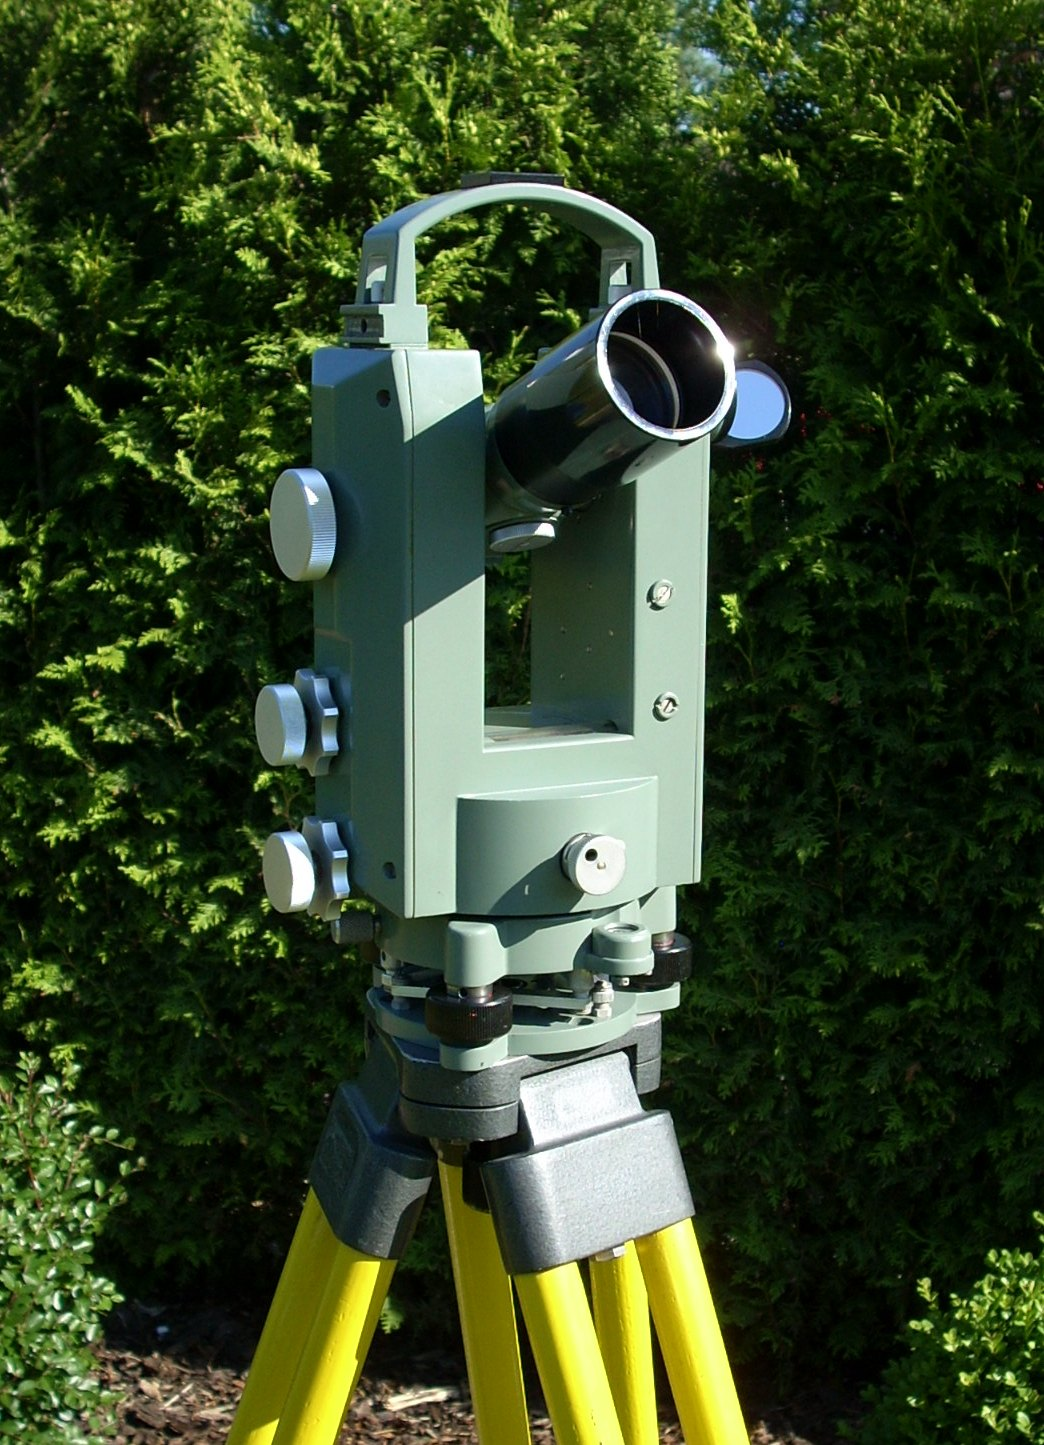
\includegraphics[width=.5\linewidth]{3_gonio_complexe_getallen/inputs/Askania_Sekunden-Theodolit_TU_e_400.jpg}
%\end{center}
%\end{figure}

(Bron figuur: \url{https://commons.wikimedia.org/wiki/File:Askania_Sekunden-Theodolit_TU_e_400.jpg})\\

De staalconstructie van een hoogspanningsmast is gebaseerd op driehoeken.

\gewonefiguur{height=7cm}{3_gonio_complexe_getallen/inputs/Pylon_ds.jpg}

%\begin{figure}[h]
%\begin{center}
%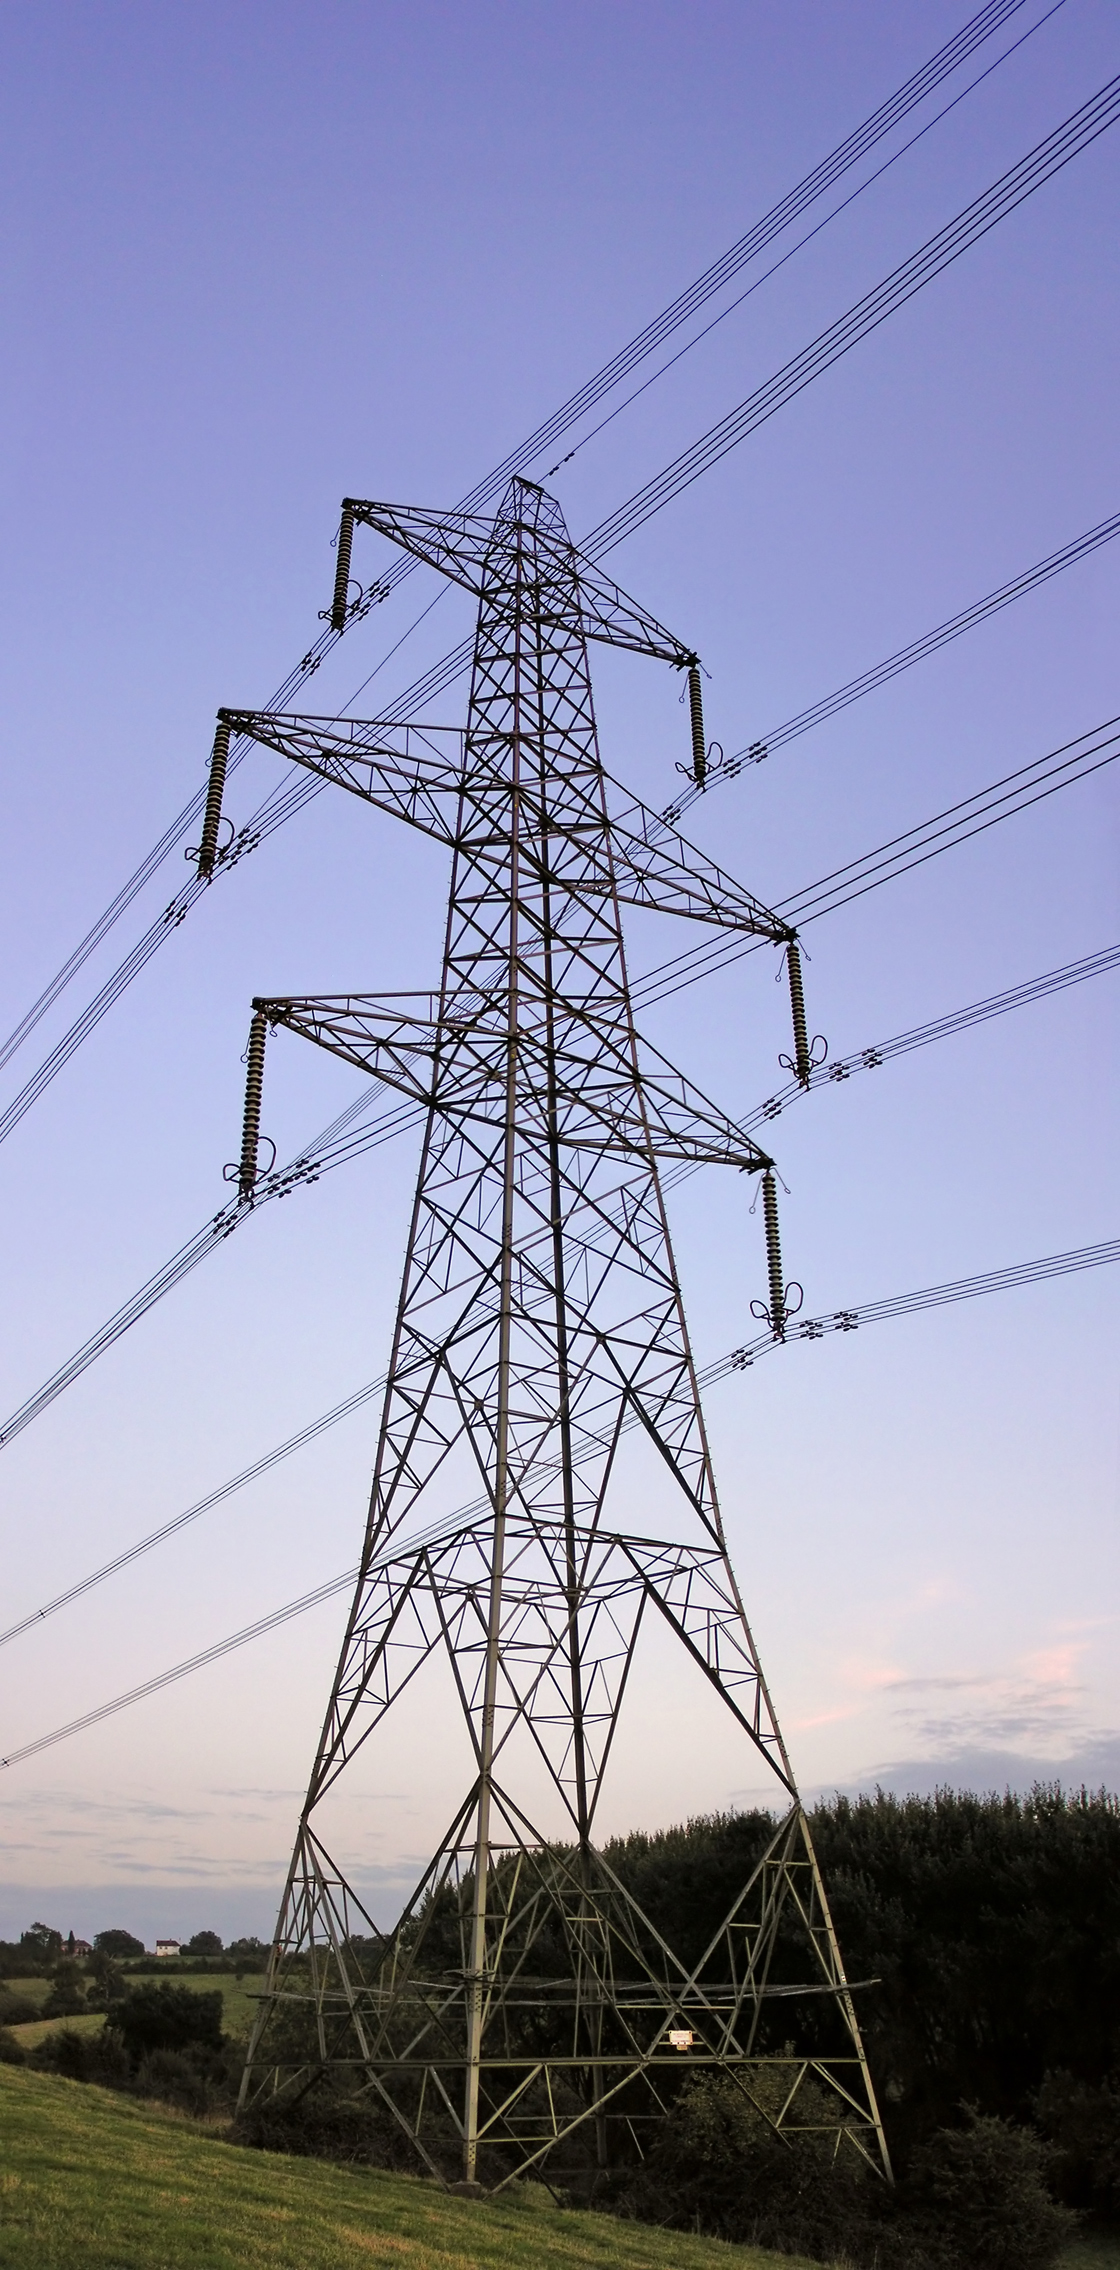
\includegraphics[width=.5\linewidth]{3_gonio_complexe_getallen/inputs/Pylon_ds.jpg}
%\end{center}
%\end{figure}

(Bron figuur: \url{https://commons.wikimedia.org/wiki/File:Pylon_ds.jpg}).\\

In de volgende paragrafen bespreken we praktisch de basis van goniometrie en driehoeksmeetkunde.\\

\subsection{Meten van hoeken}

%\begin{itemize}
%	\item Wat zijn de verschillende manieren om hoeken te meten?
%	\item Hoe kan je overgaan van de ene hoekmaat naar de andere?
%\end{itemize}

\subsubsection{Graden, minuten, seconden}

Een hoekmaat wordt bepaald door een hoek voor te stellen op een cirkel met willekeurige straal $r$ waarbij men de top van de hoek laat samenvallen met het middelpunt van de cirkel. Elke hoek $\alpha$ komt dan overeen met een zekere afstand gemeten langs de omtrek van de cirkel. Men zegt dat met elke hoek $\alpha$ een zekere booglengte op de cirkel met straal $r$ overeenkomt.

\gewonefiguur{scale=.5}{3_gonio_complexe_getallen/inputs/goncirkelhoek-1.pdf}

%\begin{figure}[h]
%\begin{center}
%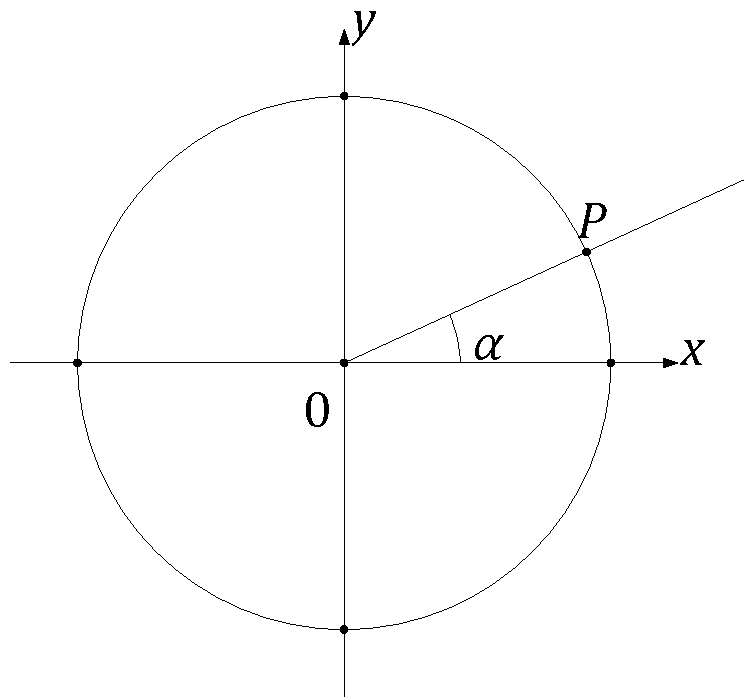
\includegraphics[scale=.5]{3_gonio_complexe_getallen/inputs/goncirkelhoek-1.pdf}
%\end{center}
%\end{figure}

Door nu de cirkelomtrek onder te verdelen in allemaal stukjes met gelijke booglengte bekomt men een maat voor een hoek. Op de figuur hieronder zijn enkele onderverdelingen getekend.

\gewonefiguur{scale=.37}{3_gonio_complexe_getallen/inputs/graden1.jpg}

%\begin{figure}[h]
%\begin{center}
%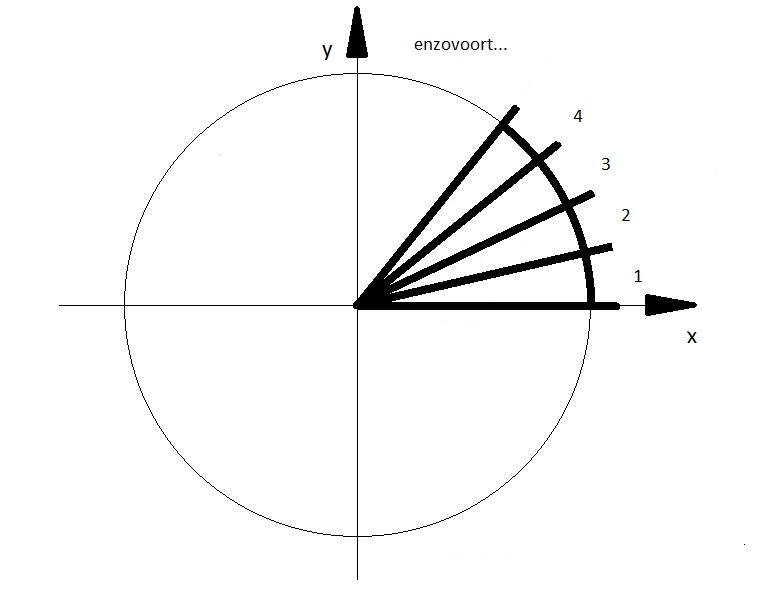
\includegraphics[scale=.37]{3_gonio_complexe_getallen/inputs/graden1.jpg}
%\end{center}
%\end{figure}

Deze onderverdelingen noemt men graden. Meestal (maar niet altijd!) wordt een cirkel onderverdeeld in $360^\circ$: een rechte hoek komt dan overeen met $90^\circ$ en een gestrekte hoek met $180^\circ$. Hieronder staan enkele tekeningen:

\gewonefiguur{scale=.5}{3_gonio_complexe_getallen/inputs/hoekendeg.pdf}

%\begin{figure}[h]
%\begin{center}
%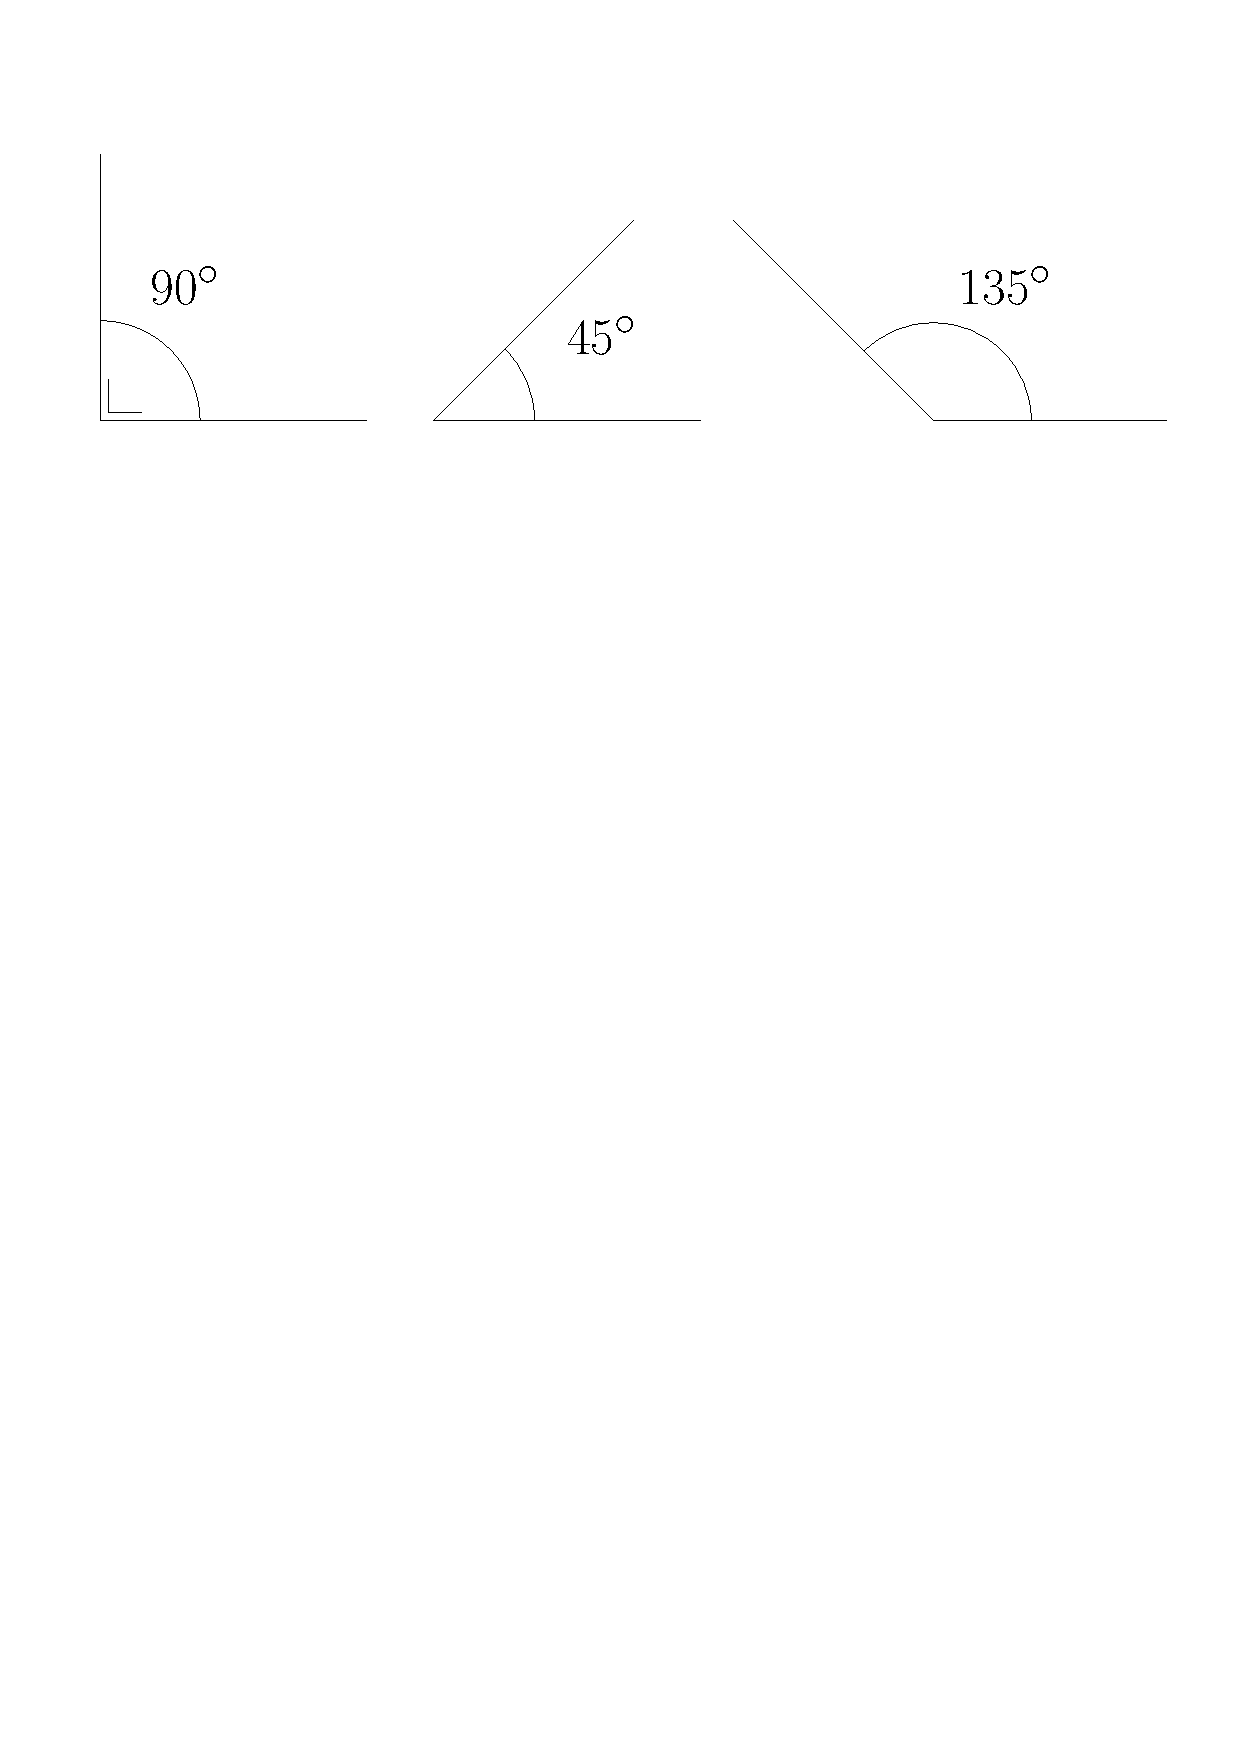
\includegraphics[scale=.5]{3_gonio_complexe_getallen/inputs/hoekendeg.pdf}
%\end{center}
%\end{figure}

Graden zijn zelf ingedeeld in minuten (zoals meters kunnen ingedeeld worden in centimeters) en minuten kunnen op hun beurt worden ingedeeld in seconden (zoals centimeters kunnen worden ingedeeld in millimeters).  Graden, minuten en seconden worden echter ingedeeld in een $60$-tallig talstelsel, waardoor je volgende regels krijgt:

\begin{align*}
	1 \textrm{ graad} &= 60 \textrm{ minuten}\\
	1 \textrm{ minuut} &= 60 \textrm{ seconden}
\end{align*}

Deze hoekmaat noemt men de zestigdelige graad. De zestigdelige graad wordt soms afgekort als 'deg' van het Engelse woord 'degree'.\\
Graden, minuten en seconden hebben hun eigen eenheid/symbool, zoals het symbool voor centimeter 'cm' is:

\begin{align*}
	1 \textrm{ graad} &= 1^\circ\\
	1 \textrm{ minuut} &= 1'\\
	1 \textrm{ seconde} &= 1''
\end{align*}

Enkele voorbeelden:

\begin{itemize}
	\item Een hoek van $1^\circ$ lees je als een hoek van '$1$ graad'. Ze bestaat zelf uit $1\cdot 60 = 60$ minuten (want elke graad is $60$ minuten), of uit $60 \cdot 60 = 3600$ seconden (want elke minuut is $60$ seconden).
	\item Een hoek van $42^\circ$ lees je dus als '$42$ graden' en bestaat zelf uit $42 \cdot 60 = 2520$ minuten (want elke graad is $60$ minuten), of uit $2520 \cdot 60 = 151200$ seconden (want elke minuut is $60$ seconden).
	\item Een hoek van $5^\circ12'13"$ lees je als $5$ graden, $12$ minuten en $13$ seconden.
\end{itemize}

Soms wordt het gebruik van minuten en seconden vermeden in de notatie van een hoek, en gebruikt men een decimale notatie. Zo kan het zijn dat je een hoek tegenkomt die genoteerd is als:
\[22,5^\circ \quad \textup{ of ook } \quad 22^\circ,5\]
Dat betekent dan ook letterlijk $22$ en een halve graad. Ofwel $22$ graden en de helft van $60$ minuten. Met andere woorden:
\[22,5^\circ = 22^\circ30'\]
Een tweede, iets moeilijker voorbeeld:

\begin{align*}
42,21^\circ &= 42^\circ+0,21\cdot 1^\circ &\textup{\footnotesize herschrijven van een kommagetal}\\
&= 42^\circ + 0,21 \cdot 60' &\textup{\footnotesize 1 graad is 60 minuten}\\
&= 42^\circ + 12,6' &\textup{\footnotesize uitrekenen}\\
&= 42^\circ + 12' + 0,6\cdot 1' &\textup{\footnotesize herschrijven van een kommagetal}\\
&= 42^\circ + 12' + 0,6 \cdot 60'' &\textup{\footnotesize 1 minuut is 60 seconden}\\
&= 42^\circ + 12' + 36'' & \textup{\footnotesize uitrekenen}\\
&= 42^\circ12'36''
\end{align*}
Gelukkig hebben veel rekentoestellen de mogelijkheid om graden in decimale notatie om te zetten in graden in notatie van graden, minuten, seconden. Raadpleeg daarvoor de handleiding van je rekentoestel.\\

Rekenen met graden, minuten, seconden is anders dan rekenen met tiendelige getallen.  Een voorbeeld:
\[12^\circ45'+36^\circ50'=48^\circ95'=49^\circ35'\]
Telkens als je meer dan $60$ minuten hebt, moet je het aantal graden verhogen met $1$. Net zo bij meer dan $60$ seconden, dan verhoog je het aantal minuten!

\subsubsection{Decimale graad of honderddelige graad}

Zoals eerder gezegd is de onderverdeling van een cirkel in $360^\circ$ alleen maar een afspraak. Volgens een andere conventie wordt een cirkel onderverdeeld in 400 stukjes zodat een rechte hoek overeenkomt met 100 onderverdelingen: men spreekt dan van decimale graden of honderddelige graden.
Honderddelige graden komen vooral voor in de topografie en de weg- en waterbouw. Vooral studenten bouwkunde zullen deze hoekmaat tegen komen. De eenheid van de 100-delige hoek is 'gon' (maar ook 'gr' of 'grad' komen voor). In principe is deze hoekmaat erg eenvoudig. Men start met de afspraak:
\[\textup{Een rechte hoek meet 100 gon.}\]
Bijgevolg zal een getrekte hoek $200$ gon meten, en een hoek van $45^\circ$ de helft van $100$ gon en dus $50$ gon. Honderddelige graden rekenen gemakkelijker dan $60$-delige graden.

\subsubsection{Radialen}

Een andere veel gebruikte hoekmaat is de radiaal. Men neemt een cirkel met straal $r$ en zet daarop een bepaalde hoek uit. Met deze hoek komt dan een welbepaalde booglengte $s$ op de cirkelomtrek overeen. Men zegt nu dat die hoek waarvoor de booglengte $s$ gelijk is aan de straal $r$ een hoek is van 1 radiaal.


\gewonefiguur{scale=0.37}{3_gonio_complexe_getallen/inputs/radiaal1.jpg}

%\begin{figure}[h]
%\begin{center}
%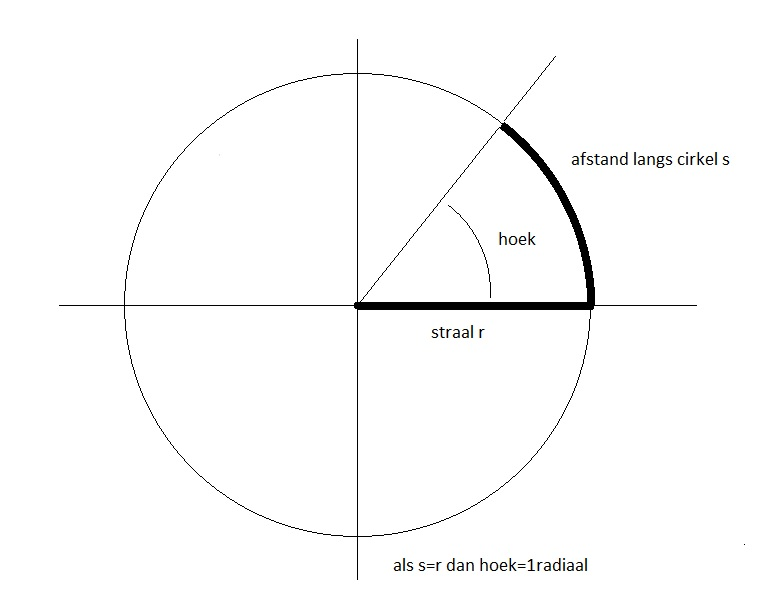
\includegraphics[scale=0.37]{3_gonio_complexe_getallen/inputs/radiaal1.jpg}
%\end{center}
%\end{figure}

Voor een hoek van 2 radialen geldt dus dat $s=2r$, voor een hoek van 5 radialen geldt dan $s=5r$, enz... M.a.w. voor een hoek $\theta$ kan men schrijven dat het verband tussen de cirkelboog $s$ en de straal $r$ gegeven wordt door:

\[ s=r\cdot \theta \]

Let op! Deze formule is all\'{e}\'{e}n geldig als de hoek $\theta$ wordt uitgedrukt in radialen...\\

In theoretische berekeningen (fysica, mechanica,...) wordt bijna altijd ondersteld dat een hoek wordt uitgedrukt in radialen zodat men van deze formule kan gebruik maken.

De omtrek van een cirkel met straal $r$ is de gekende formule $2\cdot \pi \cdot r$. Uit $s=r\cdot \theta$ volgt dan dat de hoek die overeenkomt met de volledige cirkelomtrek gelijk is aan $\theta=2\pi$. Om gemakkelijk te rekenen kiest men dikwijls een cirkel met $r=1$, de omtrek van zo een \'{e}\'{e}nheidscirkel is $2\pi$.  Met dit in het achterhoofd berekenen we de grootte van een rechte hoek ($90^\circ$), maar nu in radialen:

\gewonefiguur{scale=0.75}{3_gonio_complexe_getallen/inputs/rechtehoekrad.pdf}

%\begin{figure}[h]
%\begin{center}
%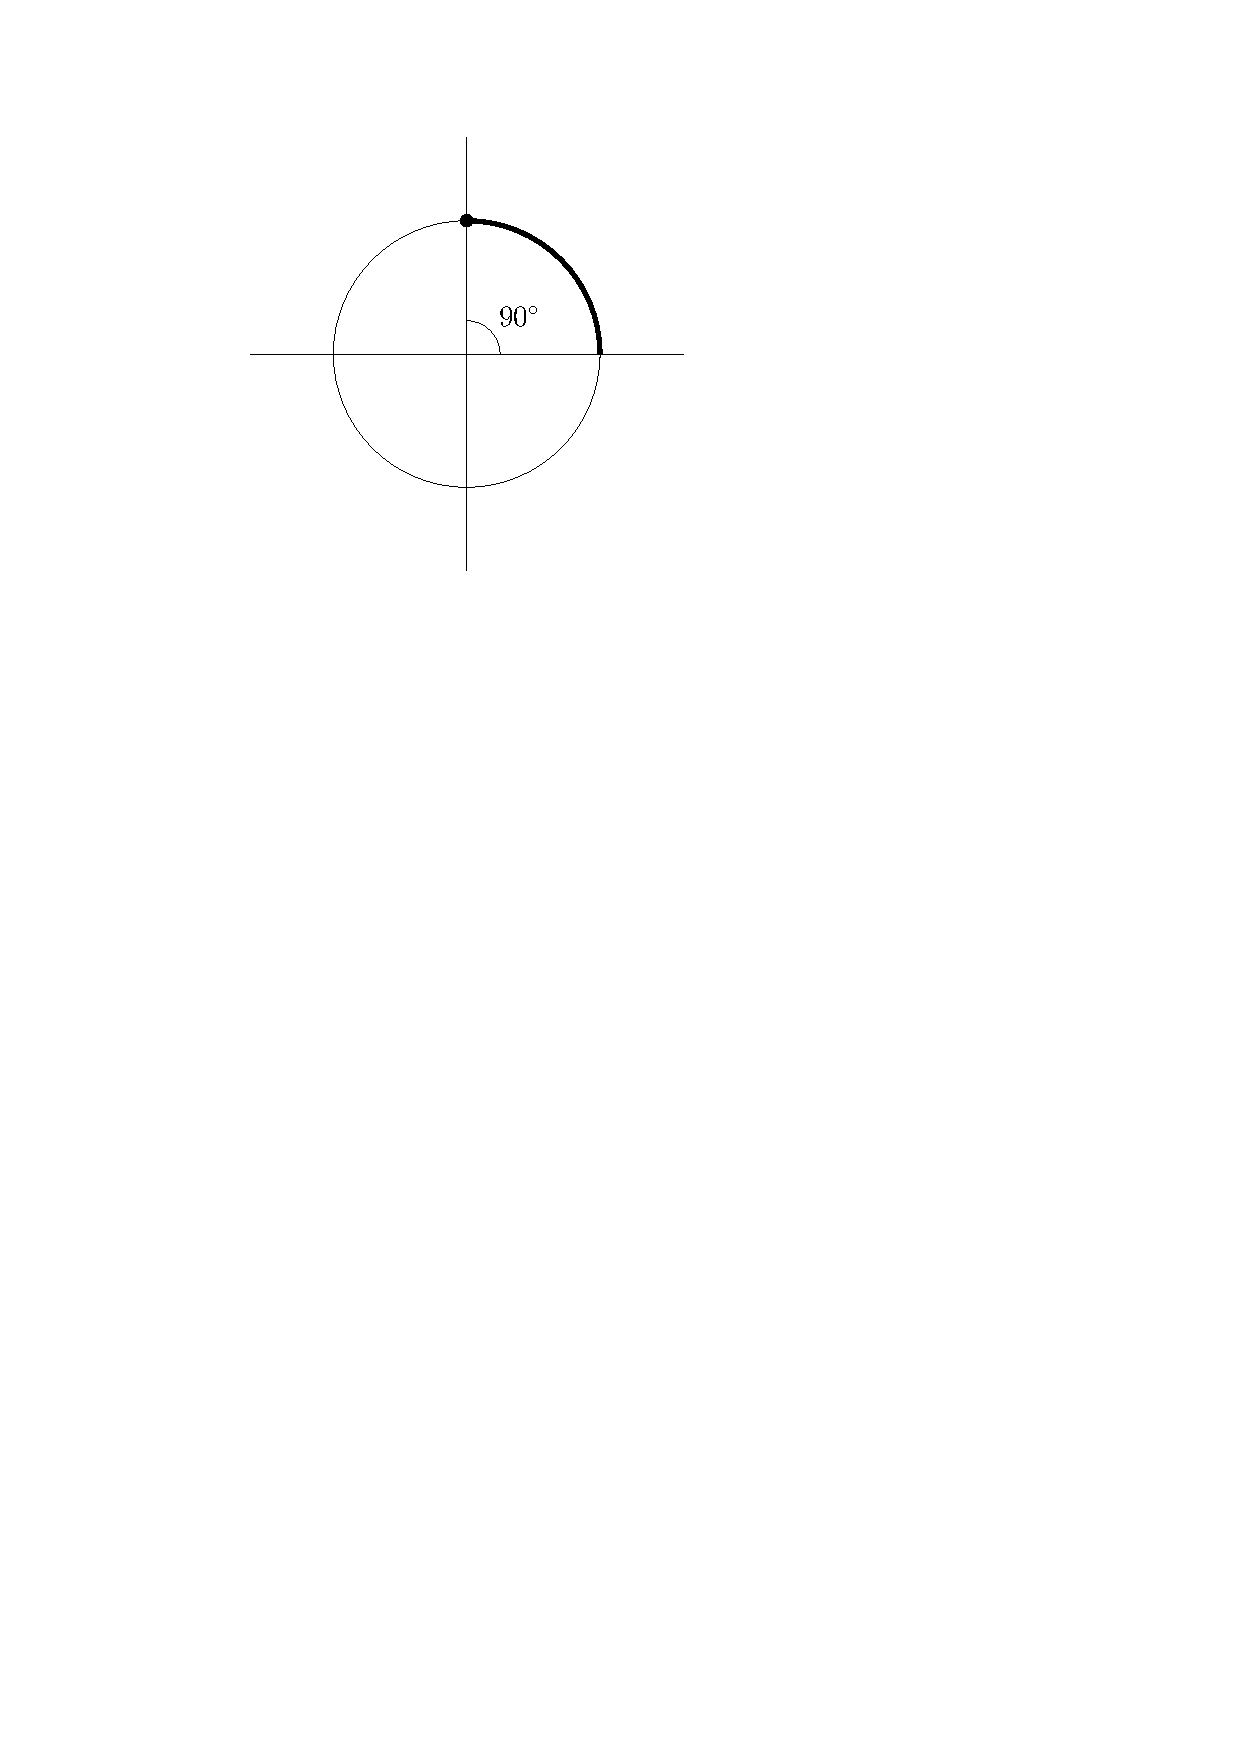
\includegraphics[scale=0.75]{3_gonio_complexe_getallen/inputs/rechtehoekrad.pdf}
%\end{center}
%\end{figure}

Je ziet dat de rechte hoek een kwart van de cirkel beslaat. De gehele cirkel heeft een omtrek van $2\pi$ en bijgevolg bepaalt de rechte hoek een cirkelboog met lengte $\dfrac{1}{4} \cdot 2\pi = \dfrac{\pi}{2}$.\\ We zeggen:

De rechte hoek meet $\dfrac{\pi}{2}$ radialen.

Op je rekentoestel worden radialen vaak aangegeven met 'rad'. Ook radialen hebben een eenheid, namelijk 'rad'. Vaak laten we deze eenheid weg:
\[90^\circ = \frac{\pi}{2} \text{rad}=\frac{\pi}{2}\]
Het voordeel van radialen is dat deze al kommagetallen zijn, en je ermee kan rekenen zoals je met gewone getallen doet. Het moeilijke is dat radialen vaak 'ongewoon' zijn, omdat het getal $\pi$ er zo vaak in opduikt.  Nog enkele veel voorkomende hoeken:
\begin{itemize}
	\item De nulhoek meet $0^\circ$ en beschrijft geen omtrek op de cirkel (het beginpunt van de cirkelboog is hetzelfde als het eindpunt ervan). Bijgevolg is de nulhoek ook een hoek van $0$ radialen.
	\item De gestrekte hoek meet $180^\circ$ en beschrijft de helft van een cirkel (tekenen!). De omtrek van een halve cirkel is $\pi$ en dus meet de gestrekte hoek $\pi$ radialen.
	\item De volle hoek meet $360^\circ$ en beschrijft de volledige cirkel. De omtrek van de volledige cirkel is $2\pi$ en dus meet de volle hoek $2\pi$ radialen.
\end{itemize}

Volgende regel is zeer belangrijk:
\[180^\circ=\pi\]

Hieruit kan je vaak snel de grootte van een eenvoudige hoek in radialen afleiden. Bijvoorbeeld:
\begin{itemize}
	\item $60^\circ$ is gelijk aan $180^\circ:3$, en dus is de hoek van $60^\circ$ gelijk aan $\dfrac{\pi}{3}$ radialen.
	\item $30^\circ$ is gelijk aan $180^\circ:6$, en dus is de hoek van $30^\circ$ gelijk aan $\dfrac{\pi}{6}$ radialen.
	\item $45^\circ$ is gelijk aan $180^\circ:4$, en dus is de hoek van $45^\circ$ gelijk aan $\dfrac{\pi}{4}$ radialen.
\end{itemize}

Nog even een lijstje formules, waarvan de bovenste de belangrijkste is:

\begin{align*}
180^\circ&=\pi\\
360^\circ&=2\pi\\
90^\circ&=\frac{\pi}{2}\\
60^\circ&=\frac{\pi}{3}\\
45^\circ&=\frac{\pi}{4}\\
30^\circ&=\frac{\pi}{6}
\end{align*}

\subsubsection{Overgangen tussen hoeken}

\textbf{Van graden naar radialen en terug}

Omdat $180^\circ = \pi$, zal $1^\circ$ gelijk zijn aan $\dfrac{180^\circ}{180}=\dfrac{\pi}{180}$. Je kan dit gebruiken om een willekeurige hoek in graden om te zetten in radialen:
\[32^\circ = 32\cdot 1^\circ = 32 \cdot \frac{\pi}{180} \text{rad}\approx \frac{32\cdot 3,14}{180}\text{rad}=0,56\text{rad}\]
Het is wel erg belangrijk dat je een hoek in graden eerst omzet in een decimale notatie, en niet met minuten en seconden erbij. De regel wordt nu:
\begin{equation*}
x^\circ \textup{ is gelijk aan } x\cdot \frac{\pi}{180} \text{rad}
\end{equation*}
of met andere woorden, omzetten van \textbf{graden naar radialen} is vermenigvuldigen met
\begin{equation*}
\dfrac{\pi}{180}\text{rad}\approx 0,0175\text{rad}
\end{equation*}

Nog een voorbeeldje:
\[42^\circ12'36''=42,21^\circ\approx 42,21 \cdot 0,0175 \text{rad}\approx 0,74 \text{rad}\]

Omdat $\pi \text{rad} = 180^\circ$, vind je dat $1 \text{rad} = \dfrac{\pi}{\pi}=\dfrac{180^\circ}{\pi}$. Je kan dit gebruiken om een willekeurige hoek in radialen om te zetten in graden:
\[1,35~\text{rad} = 1,35 \cdot 1 \text{rad} = 1,35 \cdot \frac{180^\circ}{\pi}\approx \frac{1,35 \cdot 180^\circ}{3,14}\approx 77,35^\circ\]

Het resultaat is dus altijd een hoek in graden, in decimale notatie.  De algemene regel is dus
\[x \text{rad} \textup{ is gelijk aan } x\cdot \frac{180^\circ}{\pi}\]
of met andere woorden, omzetten van \textbf{radialen naar graden} is vermenigvuldigen met
\[
\frac{180^\circ}{\pi} \approx 57,3^\circ
\]

Nog een voorbeeldje:
\[0,456 \text{rad} \approx 0,456 \cdot 57,3^\circ = 26,13^\circ\]

Merk op dat we bij deze omzettingen vaak afronden. Dat mag enkel als het voor de opgave mag, soms moet je nauwkeurig en symbolisch werken, en dan gebruik je de formules zonder afronden!

\textbf{Van graden naar gon en terug}

We gebruiken de regel dat $90^\circ=100$ gon, dus vind je:
\begin{align*}
1^\circ &= \frac{100 \textup{ gon}}{90}= 1,111 \textup{ gon}\\
1 \textup{ gon} &= \frac{90^\circ}{100} = 0,9^\circ
\end{align*}
Dit gebruik je om de volgende omzettingsregels te vinden:
\begin{align*}
x^\circ &= x\cdot 1,111 \textup{ gon}\\
x \textup{ gon} &= x\cdot 0,9^\circ
\end{align*}

\begin{voorbeeld}
	
\begin{itemize}
	\item $12,13^\circ = 12,13 \cdot 1,111 \textup{ gon} \approx 13,48 \textup{ gon}$.
	\item $78,85 \textup{ gon} = 78,85 \cdot 0,9^\circ \approx 70,97^\circ$
\end{itemize}

\end{voorbeeld}
Ook hier is het belangrijk dat je de decimale notatie van de graden gebruikt, en niet de notatie in minuten en seconden!

\subsubsection{Onthoud}
\ \\
\begin{onthoud}
	\begin{itemize}
	\item Hoeken kan je meten in
	
\begin{itemize}
	\item graden ($^\circ$), minuten ('), seconden ('')
	\item radialen (rad), de lengte van een cirkelboog van een cirkel met straal $1$
	\item 100-delige graden(gon)
\end{itemize}
\item $180^\circ=\pi$
\item $90^\circ=100$ gon
\end{itemize}

Volgende formules zijn zeer nuttig:
\begin{eqnarray*}
x^\circ &=& x\cdot \frac{\pi}{180} \text{rad} \approx x\cdot 0,0175 \text{rad}\\
x \text{rad} &=& x \cdot \frac{180^\circ}{\pi} \approx x \cdot 57,3^\circ\\
x^\circ &=& x \cdot \frac{10}{9} \textup{ gon} \approx x \cdot 1,111 \textup{ gon}\\
x \textup{ gon} &&= x\cdot 0,9^\circ
\end{eqnarray*}
\end{onthoud}


\subsection{Rechthoekige driehoeken}

\begin{itemize}
	\item Wat is de stelling van Pythagoras?
	\item Wat zijn de sinus, cosinus, tangens en cotangens in een rechthoekige driehoek?
	\item Hoe bereken je hoeken en zijden van een rechthoekige driehoek?
\end{itemize}

\subsubsection{Tekening en definities}

\gewonefiguur{scale=.5}{3_gonio_complexe_getallen/inputs/driehoek.pdf}

%\begin{figure}[h]
%\begin{center}
%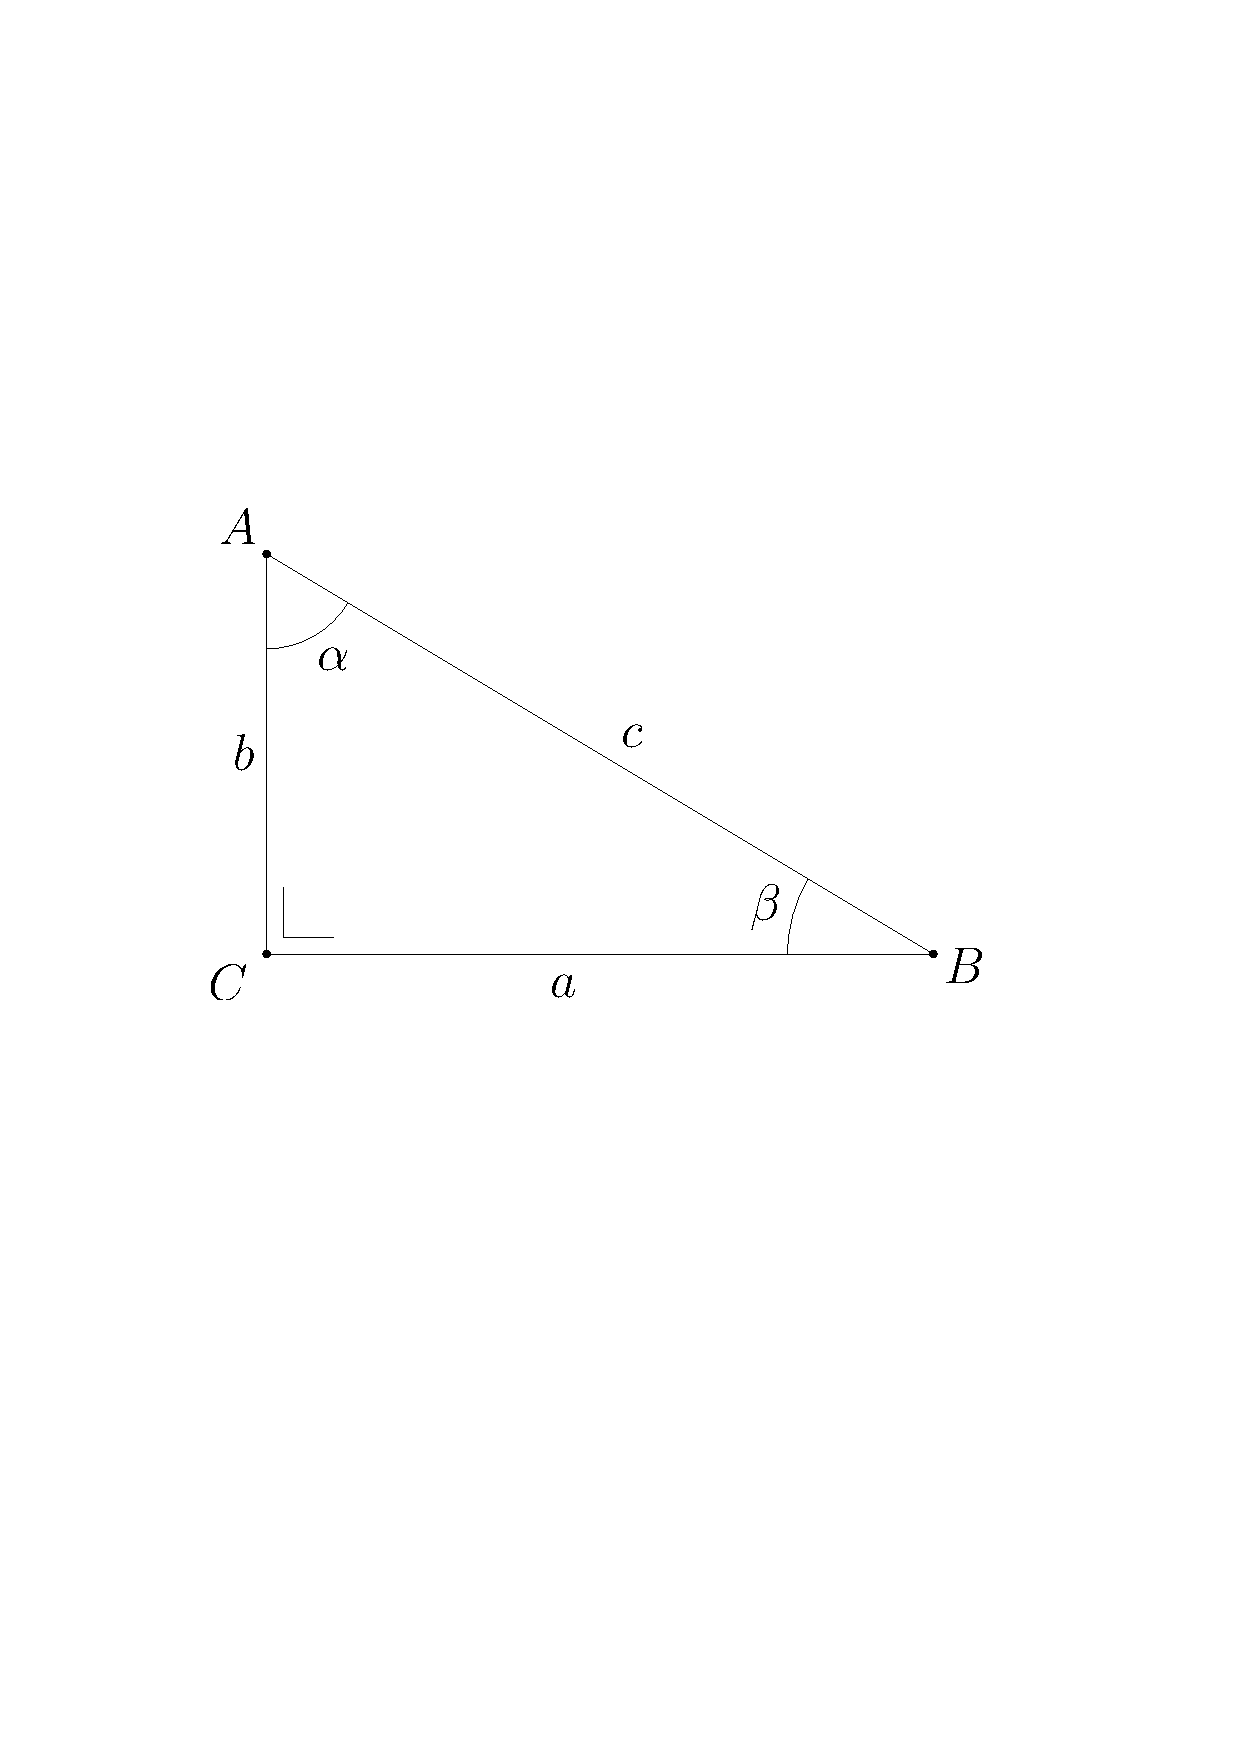
\includegraphics[scale=0.5]{3_gonio_complexe_getallen/inputs/driehoek.pdf}
%\end{center}
%\end{figure}

Een rechthoekige driehoek wordt vaak op deze manier gegeven. Een rechthoekige driehoek bestaat uit zijden en hoeken:
\begin{itemize}
	\item De zijden, aangeduid met de kleine letters $a$, $b$ en $c$.
	\item De hoekpunten $A$, $B$ en $C$.
	\item De hoeken $\alpha$ (alfa) en $\beta$ (beta).
\end{itemize}

De plaats van deze letters wordt meestal op dezelfde manier gedaan:
\begin{itemize}
	\item De rechte hoek krijgt als hoekpunt $C$. De rechte hoek krijgt vaak geen aparte naam, omdat je reeds weet dat deze $90^\circ$ is. Als ze dan toch een naam krijgt, wordt dat $\gamma$ (gamma).
	\item $\alpha$ is de hoek horende bij hoekpunt $A$, $\beta$ is de hoek horende bij hoekpunt $B$.
	\item De zijde tegenover de hoek $\alpha$ is de zijde $a$, en de zijde tegenover de hoek $\beta$ is de zijde $b$. Deze zijden noemt men de \textbf{rechthoekszijden}.
	\item De zijde $c$ ligt tegenover de rechte hoek en wordt de \textbf{hypothenusa} of \textbf{schuine zijde} genoemd.
\end{itemize}

\newpage

\subsubsection{De stelling van Pythagoras}

\begin{center}\textbf{In een rechthoekige driehoek is de 
		som van de kwadraten van de rechthoekszijden gelijk aan het kwadraat van de schuine zijde}\end{center}

\gewonefiguur{scale=.5}{3_gonio_complexe_getallen/inputs/driehoek.pdf}

%\begin{figure}[h]
%\begin{center}
%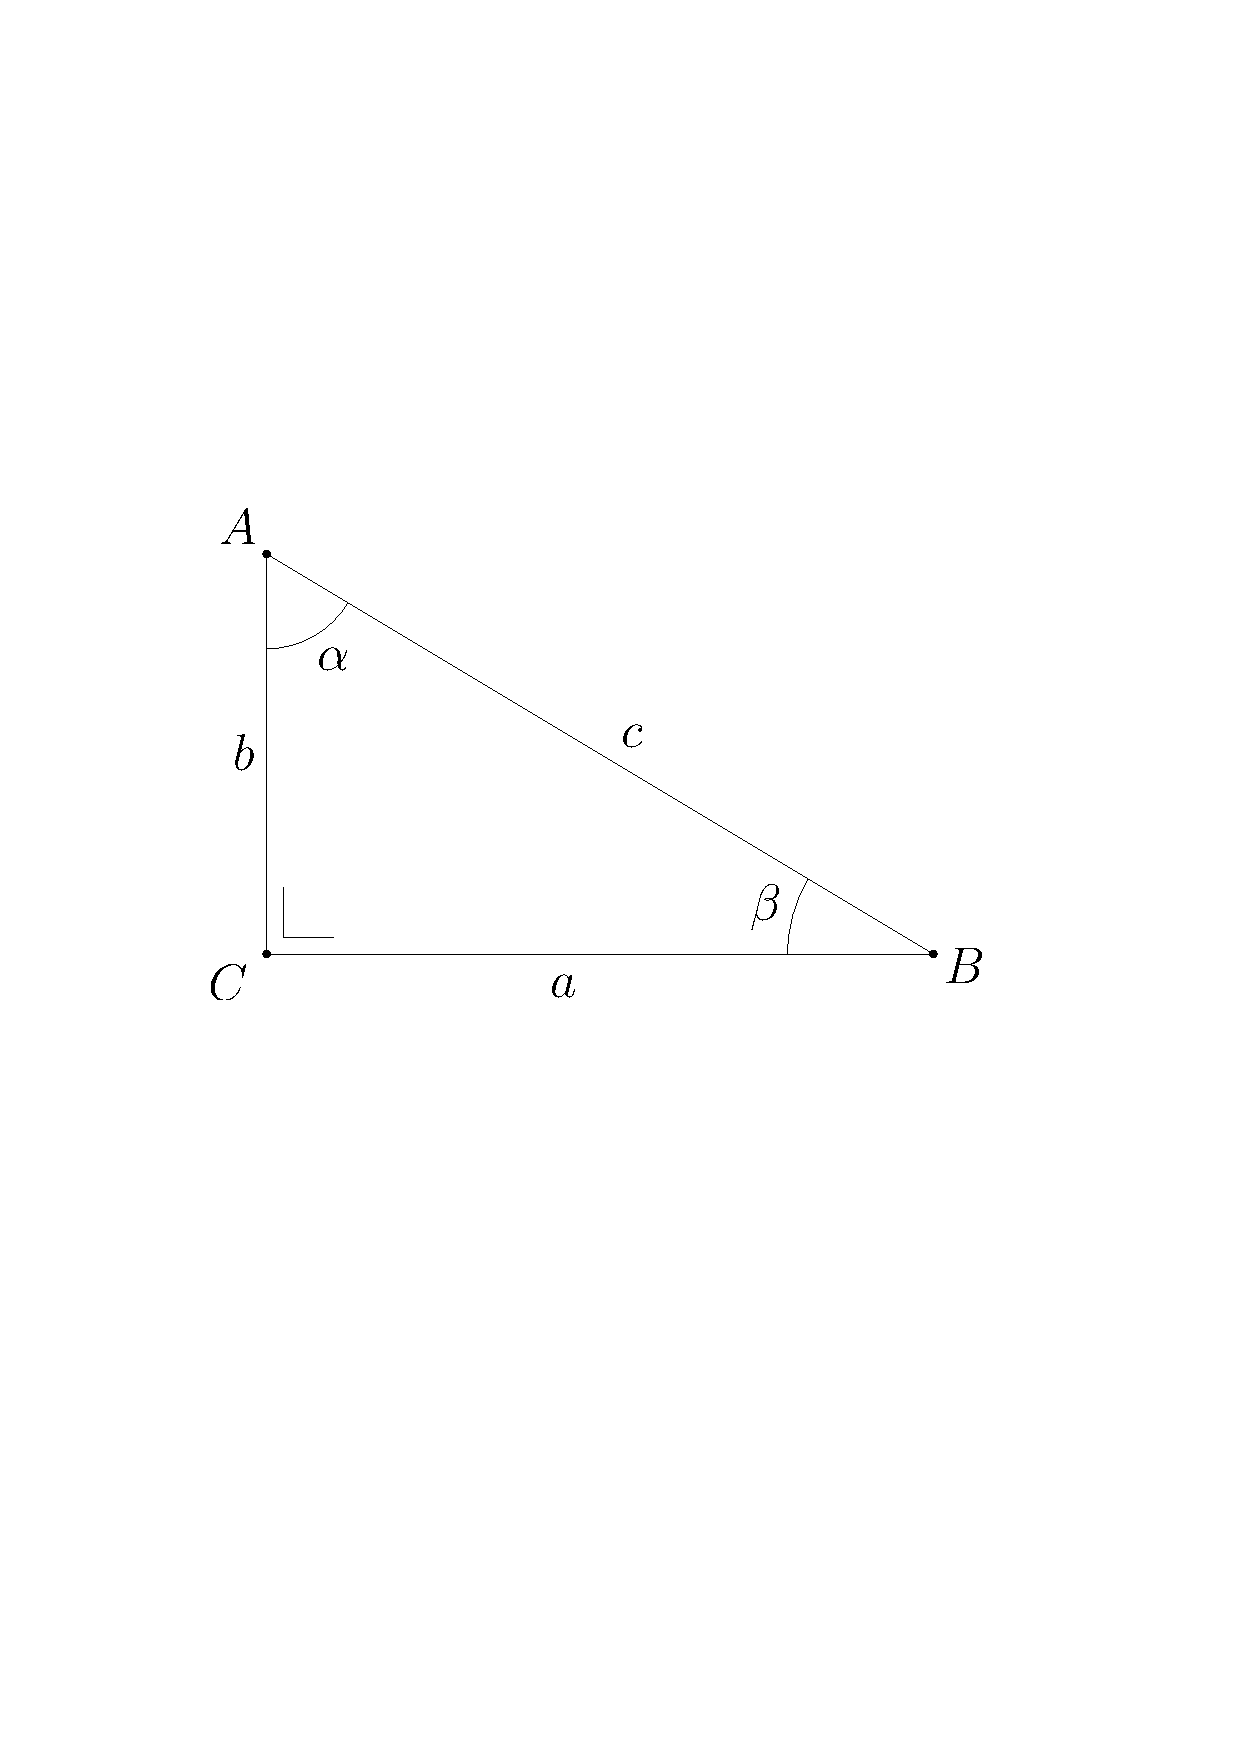
\includegraphics[scale=0.5]{3_gonio_complexe_getallen/inputs/driehoek.pdf}
%\end{center}
%\end{figure}

Voor deze tekening is dit dan:

\[a^2+b^2=c^2\]

De stelling van Pythagoras is erg nuttig om de zijden van een driehoek te berekenen. Telkens je twee zijden hebt, kan je de derde berekenen.

\subsubsection{Goniometrische getallen}

Aan een hoek $\alpha$ van een rechthoekige driehoek kunnen we een aantal getallen koppelen:
\begin{align*}
\textup{de sinus van }\alpha &=\sin \alpha &= \frac{\textup{overstaande rechthoekszijde}}{\textup{schuine zijde}}\\
&&\\
\textup{de cosinus van }\alpha &=\cos \alpha &= \frac{\textup{aanliggende rechthoekszijde}}{\textup{schuine zijde}}\\
&&\\
\textup{de tangens van }\alpha &=\tan \alpha &= \frac{\textup{overstaande rechthoekszijde}}{\textup{aanliggende rechthoekszijde}}\\
&&\\
\textup{de cotangens van }\alpha &=\cot \alpha &= \frac{\textup{aanliggende rechthoekszijde}}{\textup{overstaande rechthoekszijde}}
\end{align*}

Voor de driehoek

\gewonefiguur{scale=.5}{3_gonio_complexe_getallen/inputs/driehoek.pdf}

%\begin{figure}[h]
%\begin{center}
%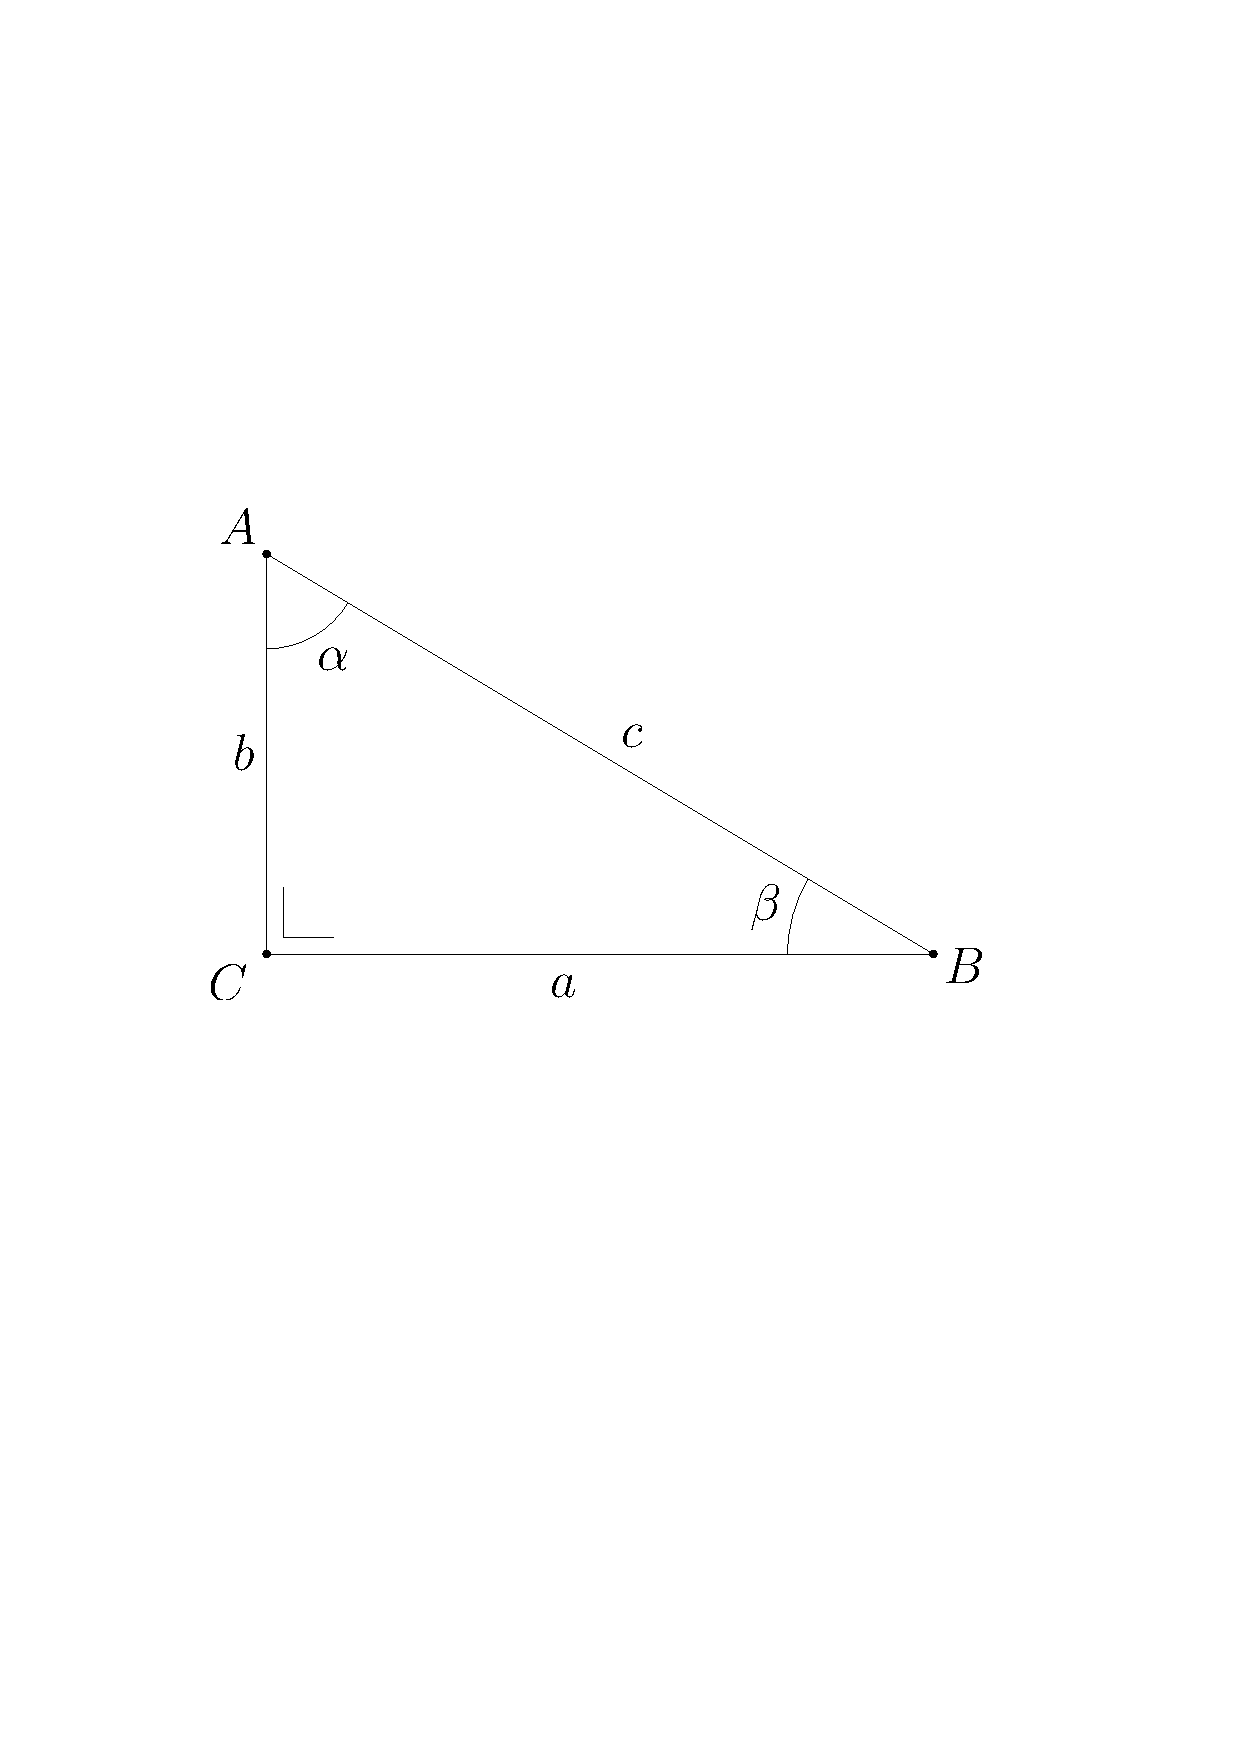
\includegraphics[scale=0.5]{3_gonio_complexe_getallen/inputs/driehoek.pdf}
%\end{center}
%\end{figure}

Is dat dan:

\begin{center}
\begin{tabular}{ccccc}
$\sin \alpha$ &$= \dfrac{a}{c}$ &\qquad\qquad\qquad& $\cos \alpha$ &$= \dfrac{b}{c}$\\
&&&&\\
$\tan \alpha$ &$= \dfrac{a}{b}$ &\qquad\qquad\qquad& $\cot \alpha$ &$= \dfrac{b}{a}$
\end{tabular}
\end{center}

Uiteindelijk zijn sinus, cosinus, \ldots van een hoek niet afhankelijk van de driehoek waar je ze in tekent. Daarom kan je ook met je rekentoestel een sinus, cosinus, \ldots berekenen. Zorg wel dat je hoekmaat juist staat ingesteld!

\subsubsection{Nuttige formules}

Volgende formules zijn vaak nuttig om hoeken terug te vinden (met $\sin^2 \alpha$ bedoelen we het kwadraat van de sinus van $\alpha$, of met andere woorden, $(\sin \alpha)^2$):

\begin{align*}
\sin^2 \alpha + \cos^2 \alpha &= 1\\
\tan \alpha &= \frac{\sin \alpha}{\cos \alpha}\\
\cot \alpha &= \frac{\cos \alpha}{\sin \alpha}\\
\tan \alpha\cdot \cot \alpha &= 1
\end{align*}

\textbf{Oplossen van rechthoekige driehoeken}


We hebben enkele formules nodig, studeer deze goed!  Voor een {\bf rechthoekige} driehoek geldt:

\gewonefiguur{scale=.5}{3_gonio_complexe_getallen/inputs/driehoek.pdf}

%\begin{figure}[h]
%\begin{center}
%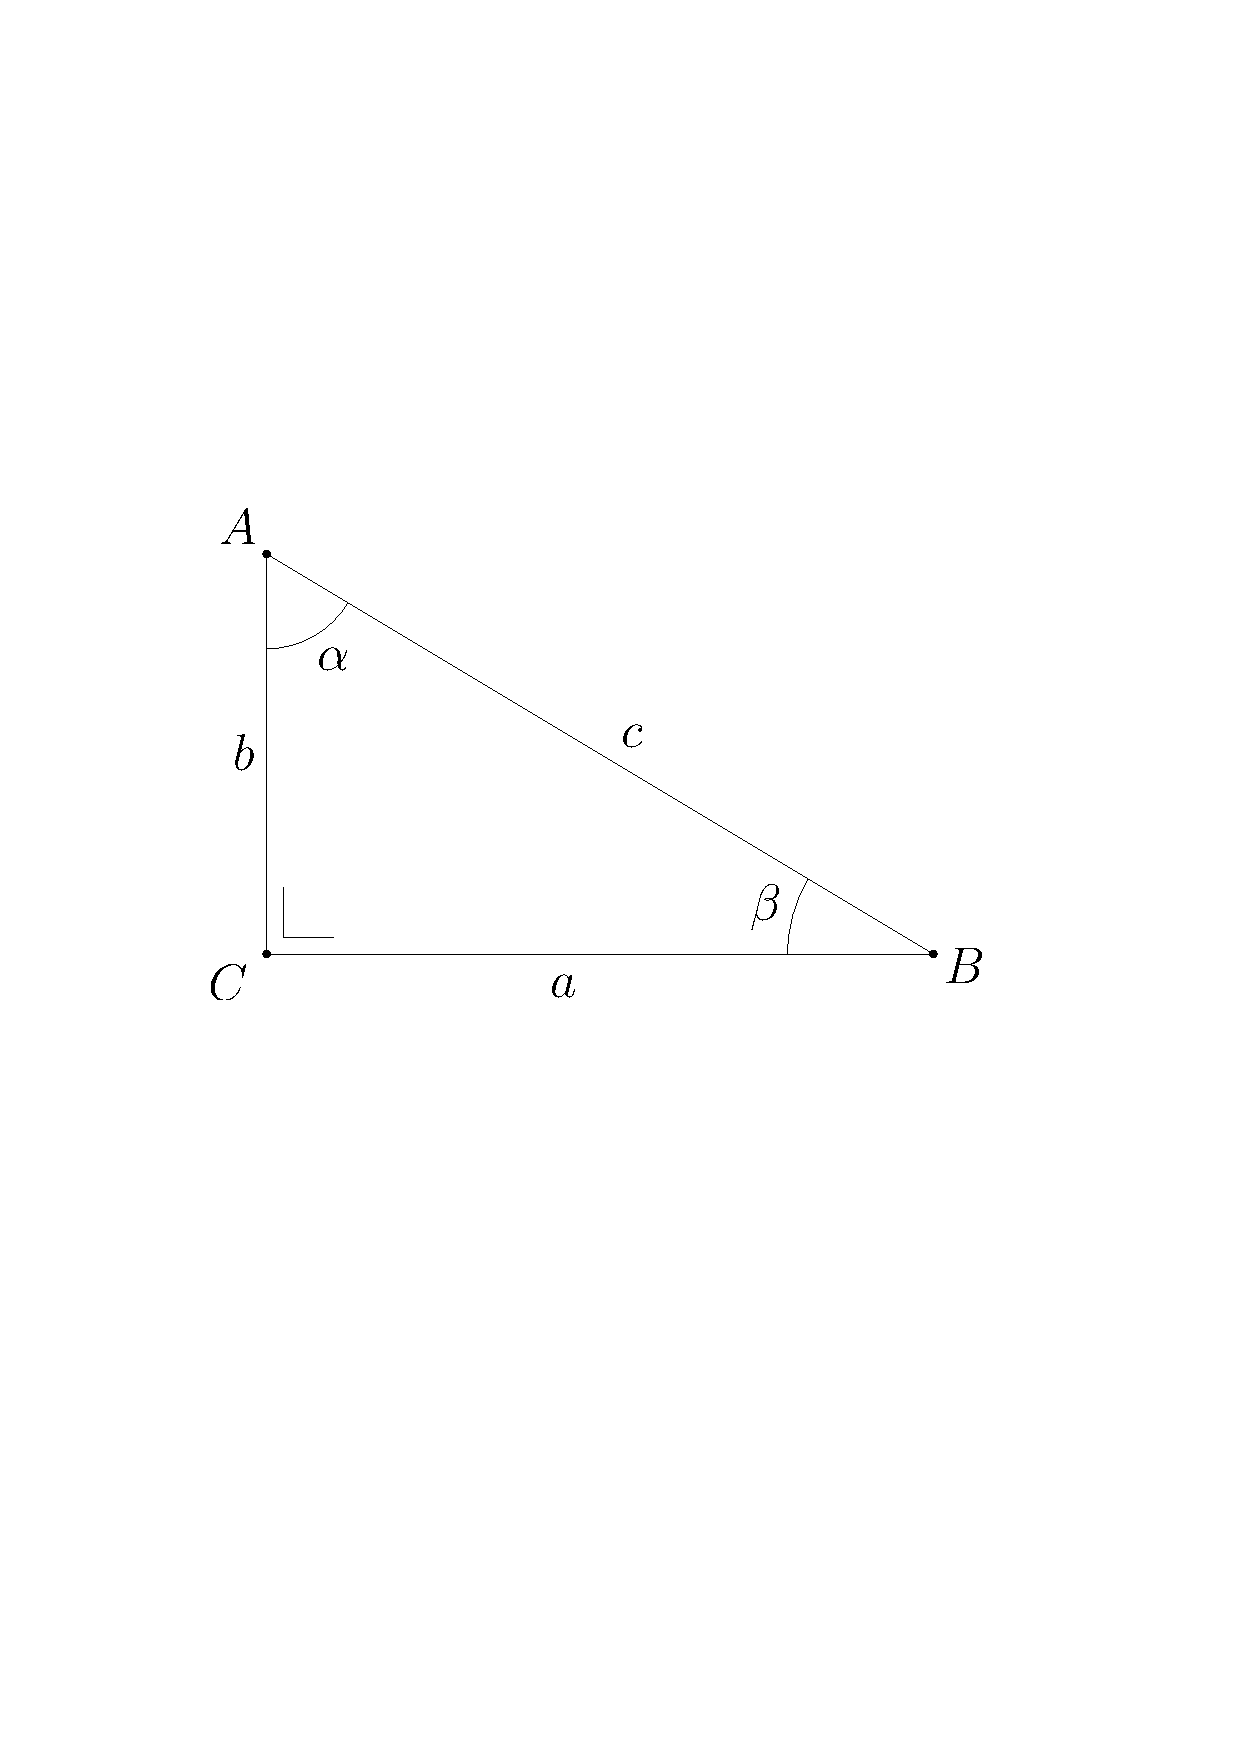
\includegraphics[scale=0.5]{3_gonio_complexe_getallen/inputs/driehoek.pdf}
%\end{center}
%\end{figure}

\begin{center}
\begin{tabular}{ccccc}
&&$a^2+b^2=c^2$ &&\\
&&&&\\
$\sin \alpha=$ & $\dfrac{a}{c}$ &\qquad\qquad\qquad & $\sin \beta=$ & $\dfrac{b}{c}$\\
&&&&\\
$\cos \alpha=$ & $\dfrac{b}{c}$ &\qquad\qquad\qquad & $\cos \beta=$ & $\dfrac{a}{c}$\\
&&&&\\
$\tan \alpha=$ & $\dfrac{a}{b}$ &\qquad\qquad\qquad & $\tan \beta=$ & $\dfrac{b}{a}$\\
\end{tabular}
\end{center}

Wat kan je hier nu mee? Als je enkele onderdelen van een rechthoekige driehoek gegeven hebt, kan je met deze formules en gegevens de andere onderdelen berekenen. Vaak heb je met $2$ gegeven waarden genoeg. Dit noemen we het oplossen van een rechthoekige driehoek. De bedoeling is $a$, $b$, $c$, $\alpha$ en $\beta$ te bepalen.

\begin{voorbeeld}
	Van de driehoek is gegeven $a = 3$ en $b = 4$. Bereken de overige getallen.\\
Met de stelling van Pythagoras vind je:
\[a^2+b^2=c^2 \Leftrightarrow 3^2+4^2=c^2 \Leftrightarrow 9+16=c^2 \Leftrightarrow 25=c^2 \Leftrightarrow c=5\]
We hebben de $3$ zijden, dus nu moeten we nog de twee hoeken berekenen. Dat doen we met sinus, cosinus, \ldots:
\[\sin \alpha = \frac{a}{c} = \frac{3}{5} = 0,6\]
Nu kan je met je rekentoestel uitrekenen wat $\alpha$ is, vaak met de toets $\sin^{-1}$. Je vindt:
\[\alpha \approx 36,87^\circ\]
Ook $\beta$ kan je vinden op deze manier:
\[\sin \beta = \frac{b}{c}=\frac{4}{5}=0,8\]
En dus
\[\beta \approx 53,13^\circ\]
Zie je dat $\alpha+\beta = 90^\circ$! Dit is geen toeval. De som van de hoeken van een driehoek is $180^\circ$. Omdat je $1$ hoek al kent, namelijk de rechte hoek van $90^\circ$, is de som van de andere $2$ $90^\circ$. Onthoud dus:

\begin{itemize}
	\item \textbf{De som van de hoeken van een driehoek is $180^\circ$}, of met andere woorden
	\[\alpha+\beta+\gamma=180^\circ\]
	\item \textbf{De som van de scherpe hoeken in een rechthoekige driehoek is $90^\circ$}, of m.a.w.
	\[\alpha+\beta = 90^\circ\]
\end{itemize}

\end{voorbeeld}

\begin{voorbeeld}
	Er is gegeven dat $\alpha = 30^\circ$ en $c$ (de schuine zijde) is $7$. Bereken de overige getallen.\\
Je kan meteen $\beta$ vinden:
\[\alpha+\beta=90^\circ \Leftrightarrow 30^\circ + \beta = 90^\circ \Leftrightarrow \beta = 60^\circ\]
De zijden bereken je via een sinus:
\[\sin \alpha = \frac{a}{c}\Leftrightarrow \sin 30^\circ = \frac{a}{7}\Leftrightarrow \frac{1}{2}=\frac{a}{7}\]
Je zondert nu $a$ af door links en rechts met $7$ te vermenigvuldigen en je krijgt:
\[a = \frac{7}{2}\]
De laatste zijde $b$ vind je nu met de stelling van Pythagoras
\[a^2+b^2=c^2 \Leftrightarrow \left(\frac{7}{2}\right)^2+b^2=7^2 \Leftrightarrow 12,25+b^2=49\]
Je zondert $b^2$ af
\[b^2=49-12,25=36,75\]
En dan neem je links en rechts de vierkantswortel
\[b=\sqrt{36,75}\approx 6,06\]
\end{voorbeeld}

De algemene truc is dus telkens een formule te kiezen waar $2$ van de symbolen bekend zijn, om zo het derde te vinden.

\subsubsection{Onthoud}
\begin{onthoud}
	\gewonefiguur{scale=.5}{3_gonio_complexe_getallen/inputs/driehoek.pdf}
%	\begin{figure}[h]
%\begin{center}
%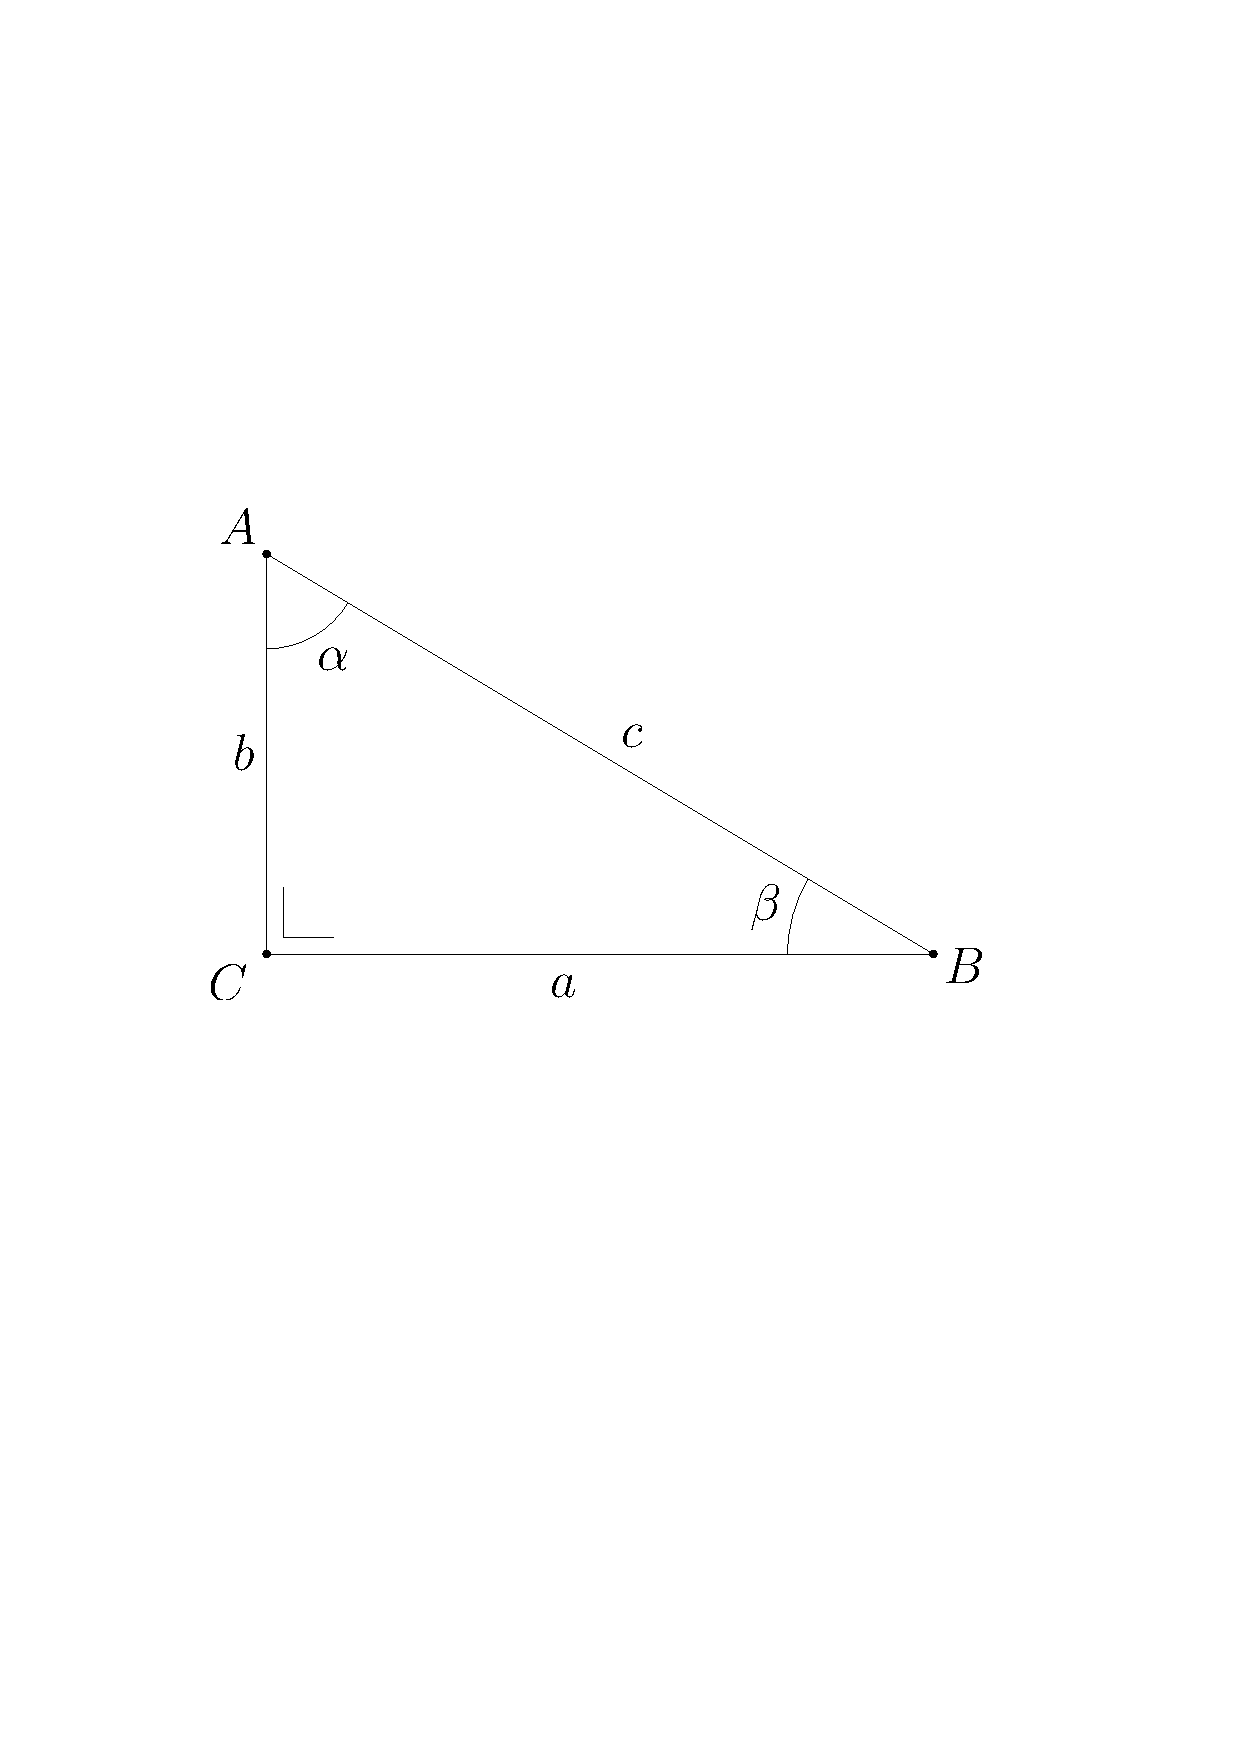
\includegraphics[scale=0.5]{3_gonio_complexe_getallen/inputs/driehoek.pdf}
%\end{center}
%\end{figure}

\begin{itemize}
	\item \textbf{De stelling van Pythagoras}
	\[a^2+b^2=c^2\]
	\item \textbf{sin, cos, tan, cot}
	\begin{center}
\begin{tabular}{ccccc}
$\sin \alpha$ &$= \dfrac{a}{c}$ &\qquad\qquad\qquad& $\cos \alpha$ &$= \dfrac{b}{c}$\\
&&&&\\
$\tan \alpha$ &$= \dfrac{a}{b}$ &\qquad\qquad\qquad& $\cot \alpha$ &$= \dfrac{b}{a}$
\end{tabular}
\end{center}
	\item $\alpha + \beta = 90^\circ$
	\item Een rechthoekige driehoek los je op door formules te kiezen uit Pythagoras, $\sin \alpha, \cos \alpha, \tan\alpha, \sin \beta, \ldots$ waarin twee waarden bekend zijn om zo de derde te vinden.
\end{itemize}
\end{onthoud}


\subsection{Willekeurige driehoeken}

%\begin{itemize}
%	\item Wat is de cosinusregel?
%	\item Wat is de sinusregel?
%	\item Hoe bereken je de zijden en hoeken van een willekeurige driehoek?
%\end{itemize}

\subsubsection{Tekening en afspraken}

\gewonefiguur{scale=.5}{3_gonio_complexe_getallen/inputs/willdriehoek.pdf}

%\begin{figure}[h]
%\begin{center}
%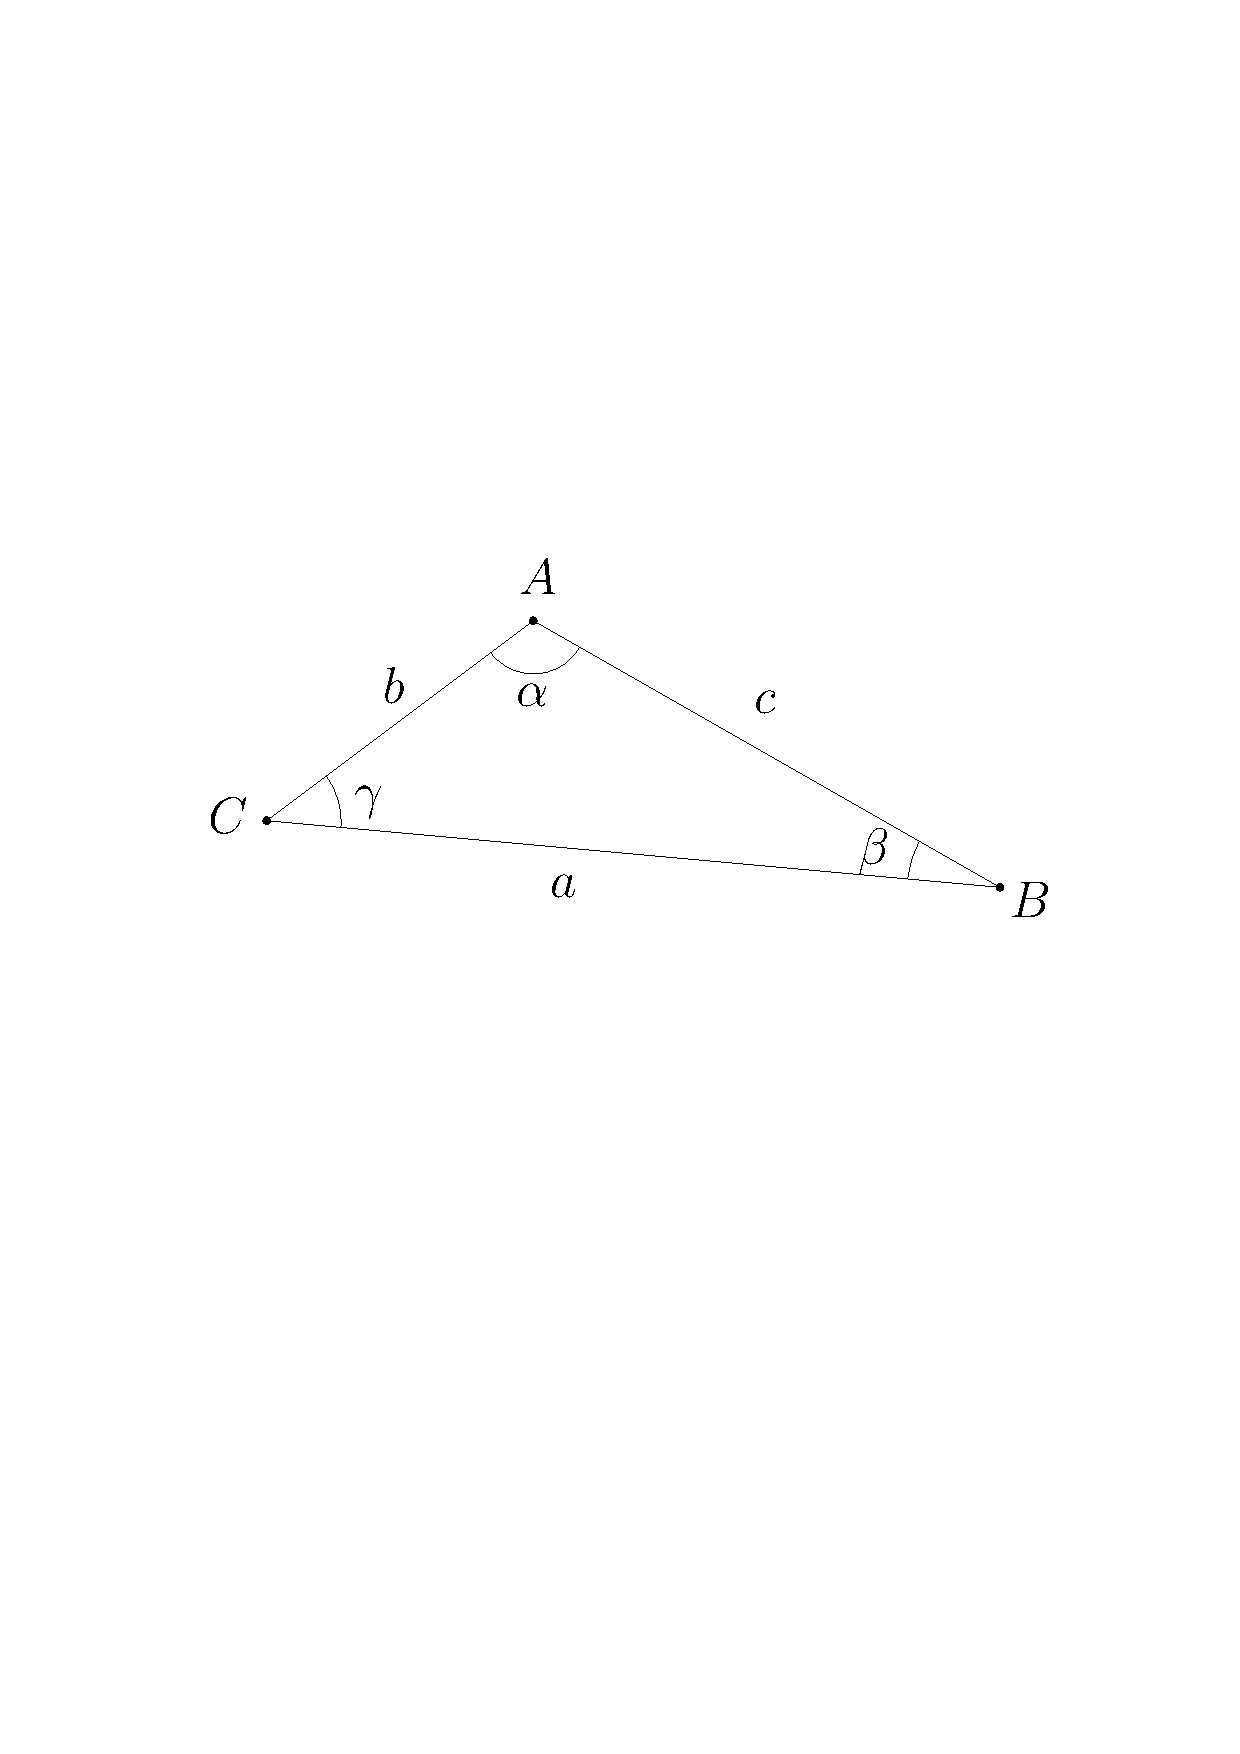
\includegraphics[scale=0.5]{3_gonio_complexe_getallen/inputs/willdriehoek.pdf}
%\end{center}
%\end{figure}

\begin{itemize}
	\item De hoekpunten duiden we aan met $A$, $B$, $C$.
	\item De bijhorende hoeken duiden we aan met $\alpha$ (alfa) bij $A$, $\beta$ (beta) bij $B$ en $\gamma$ (gamma) bij $C$.
	\item De zijde tegenover duiden we aan met $a$ (tegenover $A$), $b$ (tegenover $B$) en $c$ (tegenover $C$).
\end{itemize}

\subsubsection{Sinus- en cosinusregel}

We herinneren er nog eens aan dat de stelling van Pythagoras en de formules voor sinus, cosinus, tangens en cotangens die we tot nu toe besproken hebben all\'{e}\'{e}n geldig zijn voor rechthoekige driehoeken.\\ Voor een willekeurige driehoek gelden iets ingewikkelder formules die de sinusregel en de cosinusregel genoemd worden.\\

De \textbf{cosinusregel:}

\gewonefiguur{scale=.5}{3_gonio_complexe_getallen/inputs/willdriehoek.pdf}

%\begin{figure}[h]
%\begin{center}
%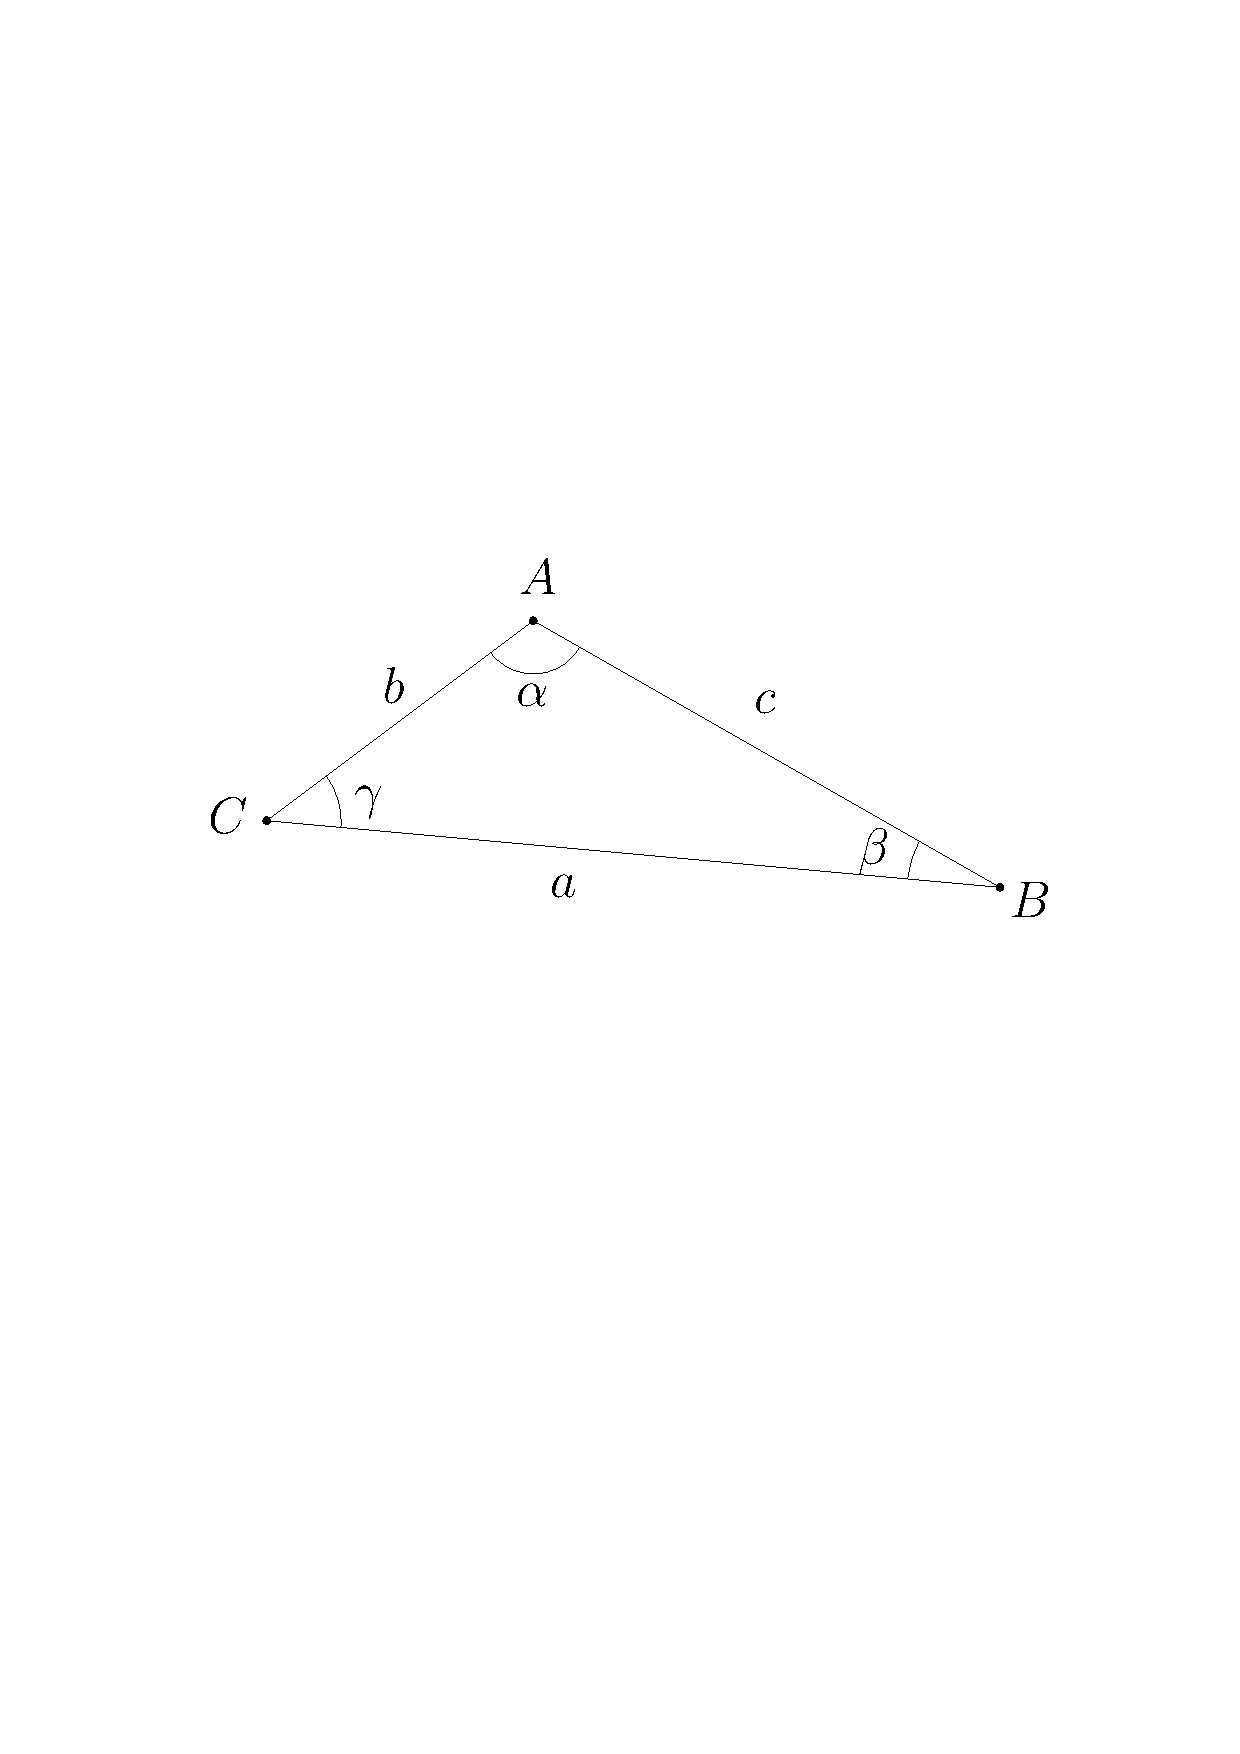
\includegraphics[scale=0.5]{3_gonio_complexe_getallen/inputs/willdriehoek.pdf}
%\end{center}
%\end{figure}

\begin{align*}
a^2&= b^2+c^2-2bc\cos \alpha\\
b^2&=a^2 + c^2 - 2ac\cos \beta\\
c^2&= a^2 + b^2 -2ab \cos \gamma
\end{align*}

Je ziet dat in het linkerlid altijd $1$ bepaalde zijde voorkomt, dat er in het rechterlid de twee andere voorkomen, samen met de cosinus van de hoek die hoort bij het linkerlid. Vergeet zeker de $-2$ niet bij de cosinus!\\

{\bf Opmerking:} als \'{e}\'{e}n van de hoeken een rechte hoek is, bijvoorbeeld de hoek $\alpha=90^\circ$, dan is $\cos \alpha =1$ en vereenvoudigt de cosinusregel tot de stelling van Pythagoras: $a^2=b^2 +c^2$.

De \textbf{sinusregel:}

\[\frac{a}{\sin \alpha}=\frac{b}{\sin \beta}=\frac{c}{\sin \gamma}\]

De sinusregel splits je meestal op in
\begin{align*}
\frac{a}{\sin \alpha} &= \frac{b}{\sin \beta}\\
\frac{a}{\sin \alpha} &= \frac{c}{\sin \gamma}\\
\frac{b}{\sin \beta} &= \frac{c}{\sin \gamma}
\end{align*}

Een andere vorm van de sinusregel is:

\begin{align*}
\frac{\sin \alpha}{a} &= \frac{\sin \beta}{b}\\
\frac{\sin \alpha}{a} &= \frac{\sin \gamma}{c}\\
\frac{\sin \beta}{b} &= \frac{\sin \gamma}{c}
\end{align*}

\subsubsection{Oplossen van willekeurige driehoeken}

Het oplossen van een willekeurige driehoek doe je op dezelfde manier als het oplossen van een rechthoekige driehoek, al zijn de formules anders.  Vergeet ook niet dat de som van de hoeken van een driehoek $180^\circ$ is! We gebruiken in dit onderdeel volgende tekening voor de aanduidingen:

\gewonefiguur{scale=.5}{3_gonio_complexe_getallen/inputs/willdriehoek.pdf}

%\begin{figure}[h]
%\begin{center}
%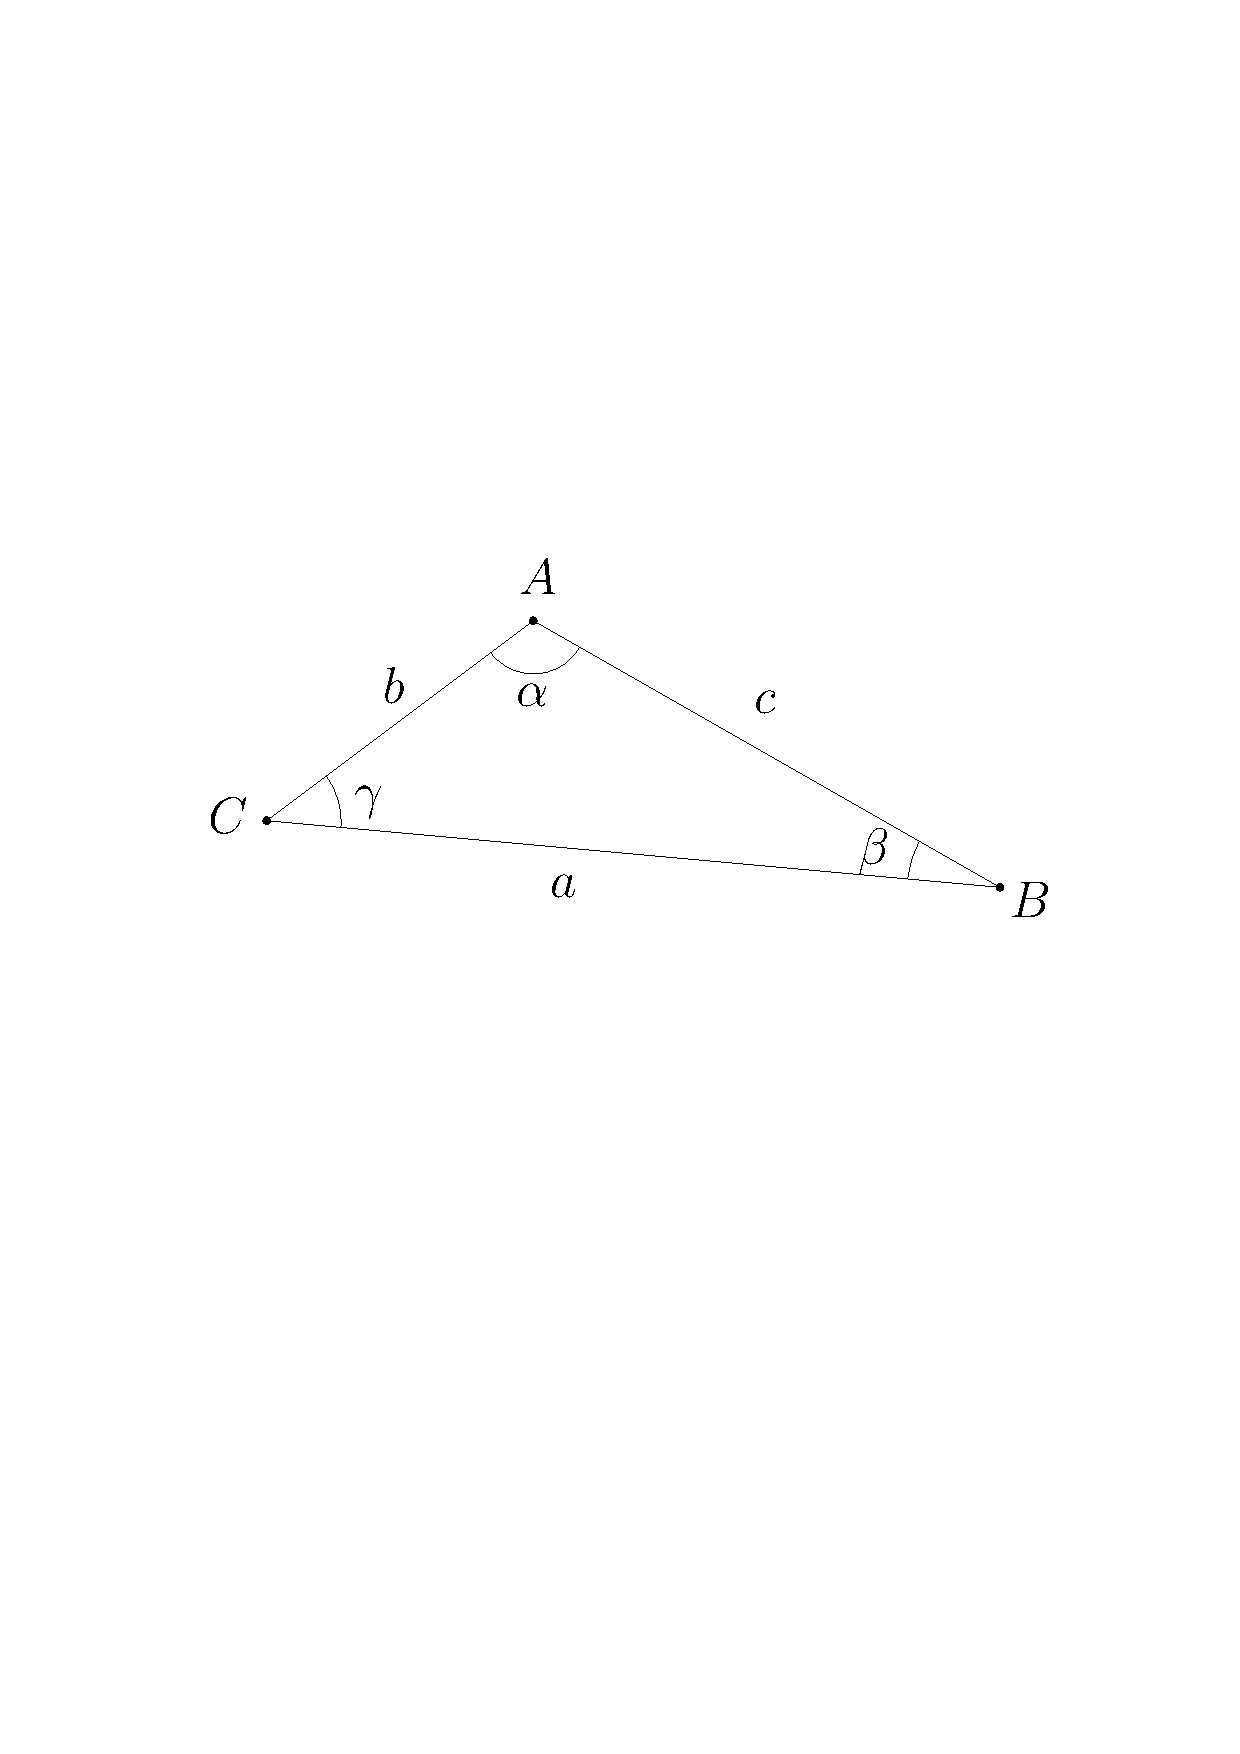
\includegraphics[scale=0.5]{3_gonio_complexe_getallen/inputs/willdriehoek.pdf}
%\end{center}
%\end{figure}

\[\alpha + \beta + \gamma = 180^\circ\]

Bij een willekeurige driehoek heb je ook meestal meer gegevens nodig dan bij een rechthoekige driehoek om hem op te lossen.  De techniek blijft hetzelfde:
\begin{center}
\textbf{Kies een formule waar $3$ onderdelen gegeven zijn, en bepaal de vierde.}
\end{center}

\begin{voorbeeld}
	In een willekeurige driehoek zijn gegeven $\alpha=20^\circ$, $\gamma = 50^\circ$ en $a=10$. Geef de andere waarden.\\
We moeten dus nog $\beta$, $b$ en $c$ berekenen. Omdat je al twee hoeken hebt, is de derde gemakkelijk te vinden uit:
\[\alpha+\beta+\gamma=180^\circ\Leftrightarrow 20^\circ + \beta + 50^\circ=180^\circ \Leftrightarrow \beta = 110^\circ\]
Om $b$ te berekenen, kunnen we de cosinusregel niet gebruiken, want we kennen $2$ zijden niet, en bij de cosinusregel treden altijd alle zijden op. Dus moeten we de sinusregel gebruiken:
\[\frac{a}{\sin \alpha} = \frac{b}{\sin \beta} = \frac{c}{\sin \gamma}\]
We kennen zowel $a$ als $\alpha$, dus gebruiken we van de sinusregel:
\[\frac{a}{\sin \alpha} = \frac{c}{\sin \gamma}\Leftrightarrow \frac{10}{\sin 20^\circ}=\frac{c}{\sin 50^\circ}\]
Je ziet dat er nog maar $1$ onbekende is, namelijk $c$.  Dus we vinden, door alles uit te rekenen:
\[\frac{10}{0,34}=\frac{b}{0,77}\Leftrightarrow c= \frac{10}{0,34}\cdot 0,77 \approx 22,65\]
Blijft er nog $b$ over, die we ook doen met de sinusregel:
\[\frac{a}{\sin \alpha}=\frac{b}{\sin \beta}\Leftrightarrow \frac{10}{0,34}=\frac{c}{0,94}\Leftrightarrow b= 27,65\]
\end{voorbeeld}

\begin{voorbeeld}
	In een willekeurige driehoek zijn gegeven $\beta = 45^\circ$, $a = 5$, $c=6$. Bepaal de andere waarden.\\
Hier hebben we slechts $1$ hoek, dus de som van de hoeken van een driehoek zal ons niet helpen. Ook met de sinusregel zijn we niet veel, omdat we teveel gegevens missen. Dus blijft er over: de cosinusregel. Welke neem je dan? Die waar $\beta$, $a$ en $c$ in staan:
\[b^2=a^2+c^2-2ac\cos\beta \Leftrightarrow b^2 = 25+36-2\cdot5\cdot 6\cos 45^\circ \Leftrightarrow b^2 = 61-60 \cdot 0,71 \approx 18,4\]
Dus neem je aan beide kanten een vierkantswortel en vind je:
\[b \approx 4,29\]
Nu je $b$ kent, en $\beta$ ook, kan je met de sinusregel $\alpha$ vinden:
\[\frac{\sin \beta}{b}=\frac{\sin \alpha}{a}\Leftrightarrow \frac{\sin 45^\circ}{4,29}=\frac{\sin \alpha}{5}\]
Afzonderen en uitrekenen, levert je dan op
\[\sin \alpha = \frac{45^\circ}{4,29}\cdot 5 = 0,82\]
Je kan nu met $\sin^{-1}$ het juiste antwoord vinden:
\[\alpha=55,08^\circ\]
$\gamma$ vind je nu met
\[\alpha+\beta+\gamma=180^\circ\Leftrightarrow 55,08^\circ + 45^\circ + \gamma = 180^\circ \Leftrightarrow \gamma = 79,92^\circ\]
\end{voorbeeld}


\begin{opmerking}
	\ \\
	
	\begin{itemize}
        \item De som van de hoeken van een driehoek is $180^\circ$, elke hoek apart heeft een grootte tussen $0^\circ$ en $180^\circ$.
		\item Bij het berekenen van de hoeken in een driehoek zal je gebruik maken van de commando's $\sin^{-1}$ en $\cos^{-1}$ op je rekentoestel. Bij gebruik van $\cos^{-1}$ zal dit de juiste hoek geven maar bij gebruik van $\sin^{-1}$ kan dit een verkeerde uitkomst geven. Dit komt omdat $\sin(180^\circ -\alpha)=\sin\alpha$ en het commando $\sin^{-1}$ steeds die hoek oplevert die kleiner is dan $90^\circ$.\\ Bijvoorbeeld: $\alpha = 45^\circ$ en $180^\circ-45^\circ = 135^\circ$ hebben dezelfde sinus. Als de onbekende hoek in de driehoek $135^\circ$ is zal $\sin^{-1}$ echter $45^\circ$ geven... \\
Praktisch ga je bij gebruik van $\sin^{-1}$ bij het oplossen van driehoeken als volgt te werk:	
	
\begin{itemize}
	\item Indien je een meetkundig correcte tekening van de driehoek hebt kan je zien of de hoek die je berekent groter of kleiner dan $90^\circ$ is. Als de hoek die je berekent met $\sin^{-1}$ groter is dan $90^\circ$ vervang dan je uitkomst $\alpha$ door $180^\circ -\alpha$.
	\item Indien je niet zeker bent van de tekening dan controleer je of de som van de hoeken van de driehoek $180^\circ$ is. Als dat niet het geval is vervang dan je uitkomst $\alpha$ door $180^\circ -\alpha$.
\end{itemize}
	
\end{itemize}
\end{opmerking}

\begin{onthoud}
	\ \\
%\begin{figure}[h]
%\begin{center}
%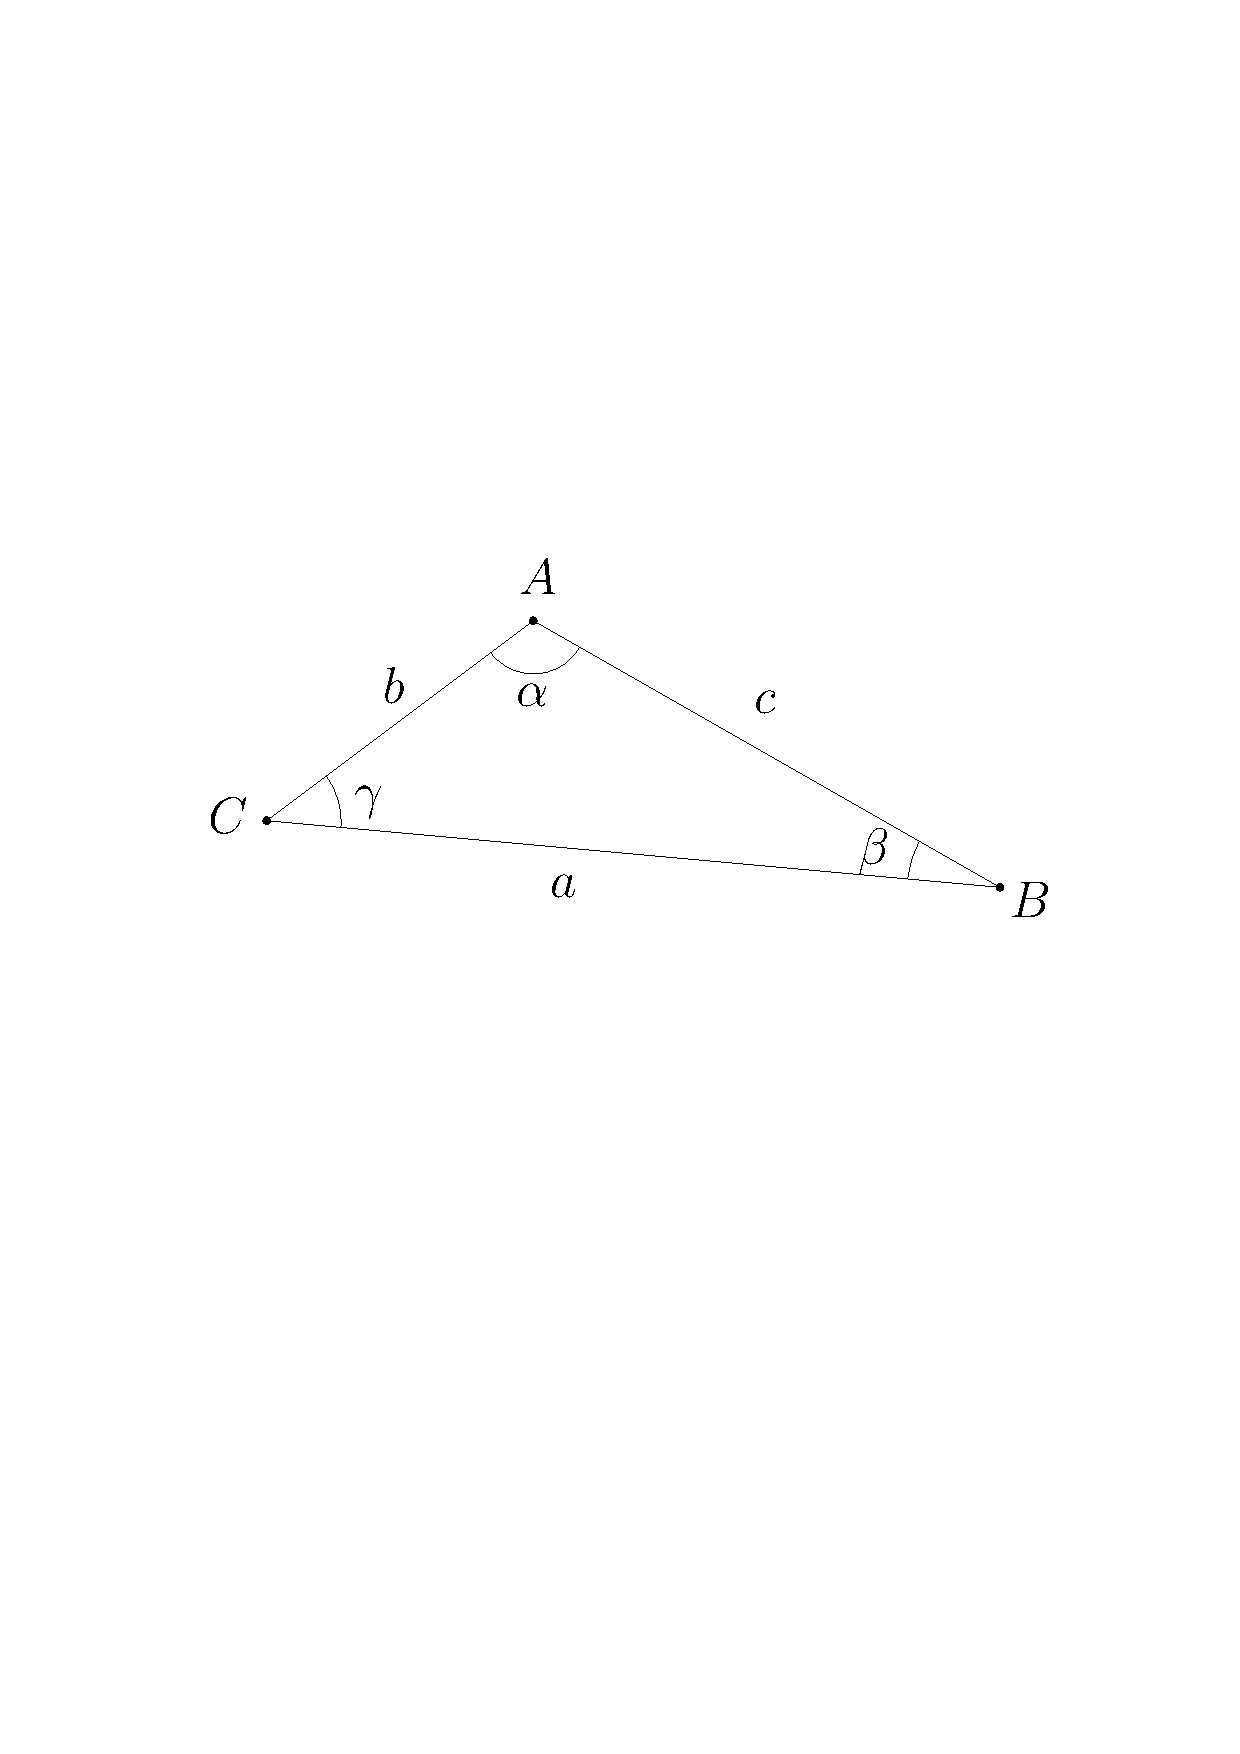
\includegraphics[scale=0.5]{3_gonio_complexe_getallen/inputs/willdriehoek.pdf}
%\end{center}
%\end{figure}

\begin{itemize}
	\item \textbf{De sinusregel}
	\[\frac{a}{\sin \alpha}=\frac{b}{\sin \beta}=\frac{c}{\sin \gamma}\]
	\item \textbf{De cosinusregel}
	\begin{align*}
a^2&= b^2+c^2-2bc\cos \alpha\\
b^2&=a^2 + c^2 - 2ac\cos \beta\\
c^2&= a^2 + b^2 -2ab \cos \gamma
\end{align*}
\item Bij het oplossen van een willekeurige driehoek, neem je best formules waar alle gegevens behalve $1$ kan ingevuld worden.
\item Pas op met de sinus en $\sin^{-1}$
\end{itemize}

\gewonefiguur{scale=.5}{3_gonio_complexe_getallen/inputs/willdriehoek.pdf}

\end{onthoud}

\subsection{De goniometrische cirkel}

%\begin{itemize}
%	\item Hoe teken je de goniometrische cirkel?
%	\item Waar bevinden zich de sinus, cosinus, tangens en cotangens op de goniometrische cirkel?
%	\item Wat zijn de kwadranten in de goniometrische cirkel?
%\end{itemize}

\subsubsection{Tekening}

In de vorige hoofdstukken hebben we de goniometrische getallen ingevoerd met een rechthoekige driehoek. We kunnen ze echter ook voorstellen op een cirkel. We tekenen een cirkel met straal $1$ door de oorsprong in een assenstelsel:
\begin{figure}[h]
\begin{center}
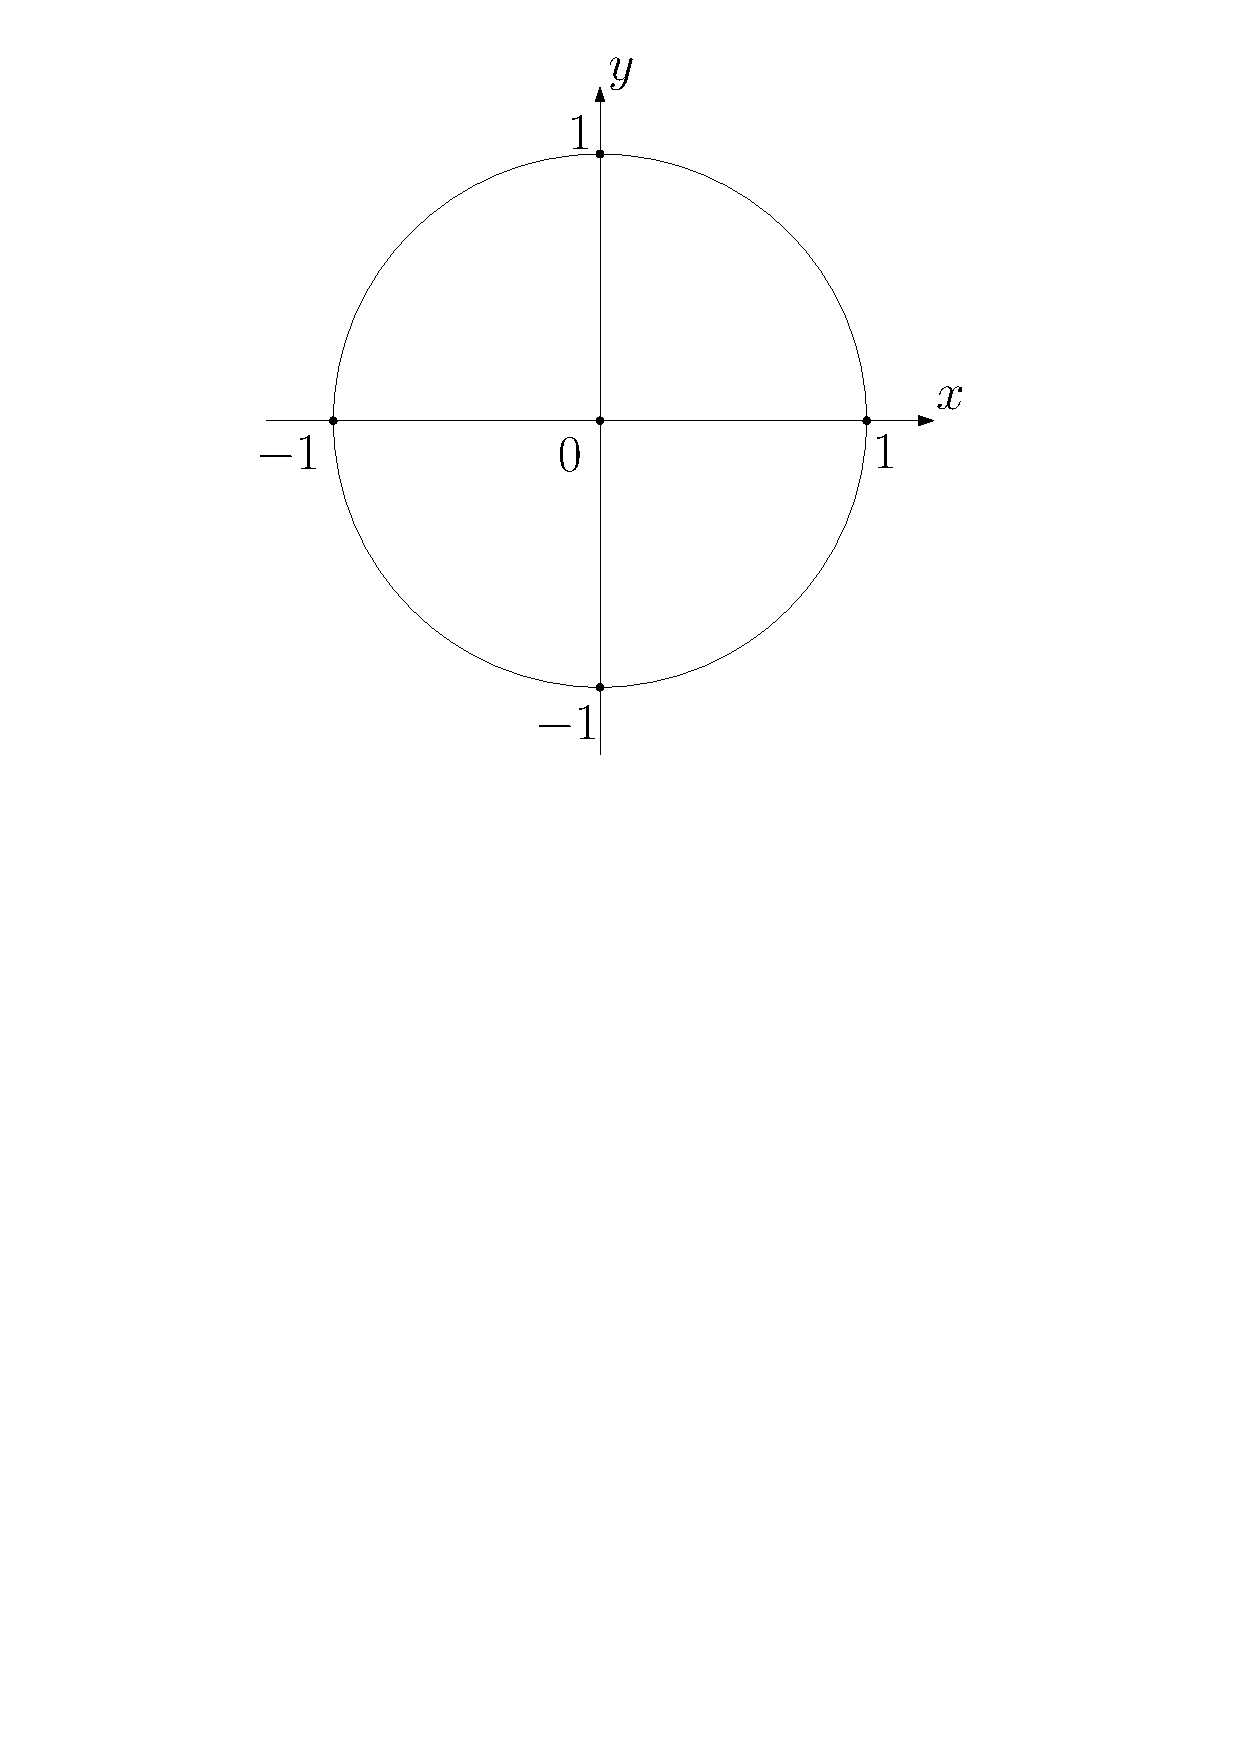
\includegraphics[scale=0.4]{3_gonio_complexe_getallen/inputs/goncirkelleeg.pdf}
\end{center}
\end{figure}

In deze cirkel kan je nu een hoek $\alpha$ tekenen, die zijn beginbeen heeft op de $x$-as, en zijn hoekpunt in de oorsprong. Zijn eindbeen snijdt de goniometrische cirkel in een punt, dat we $P$ noemen.

\begin{figure}[h]
\begin{center}
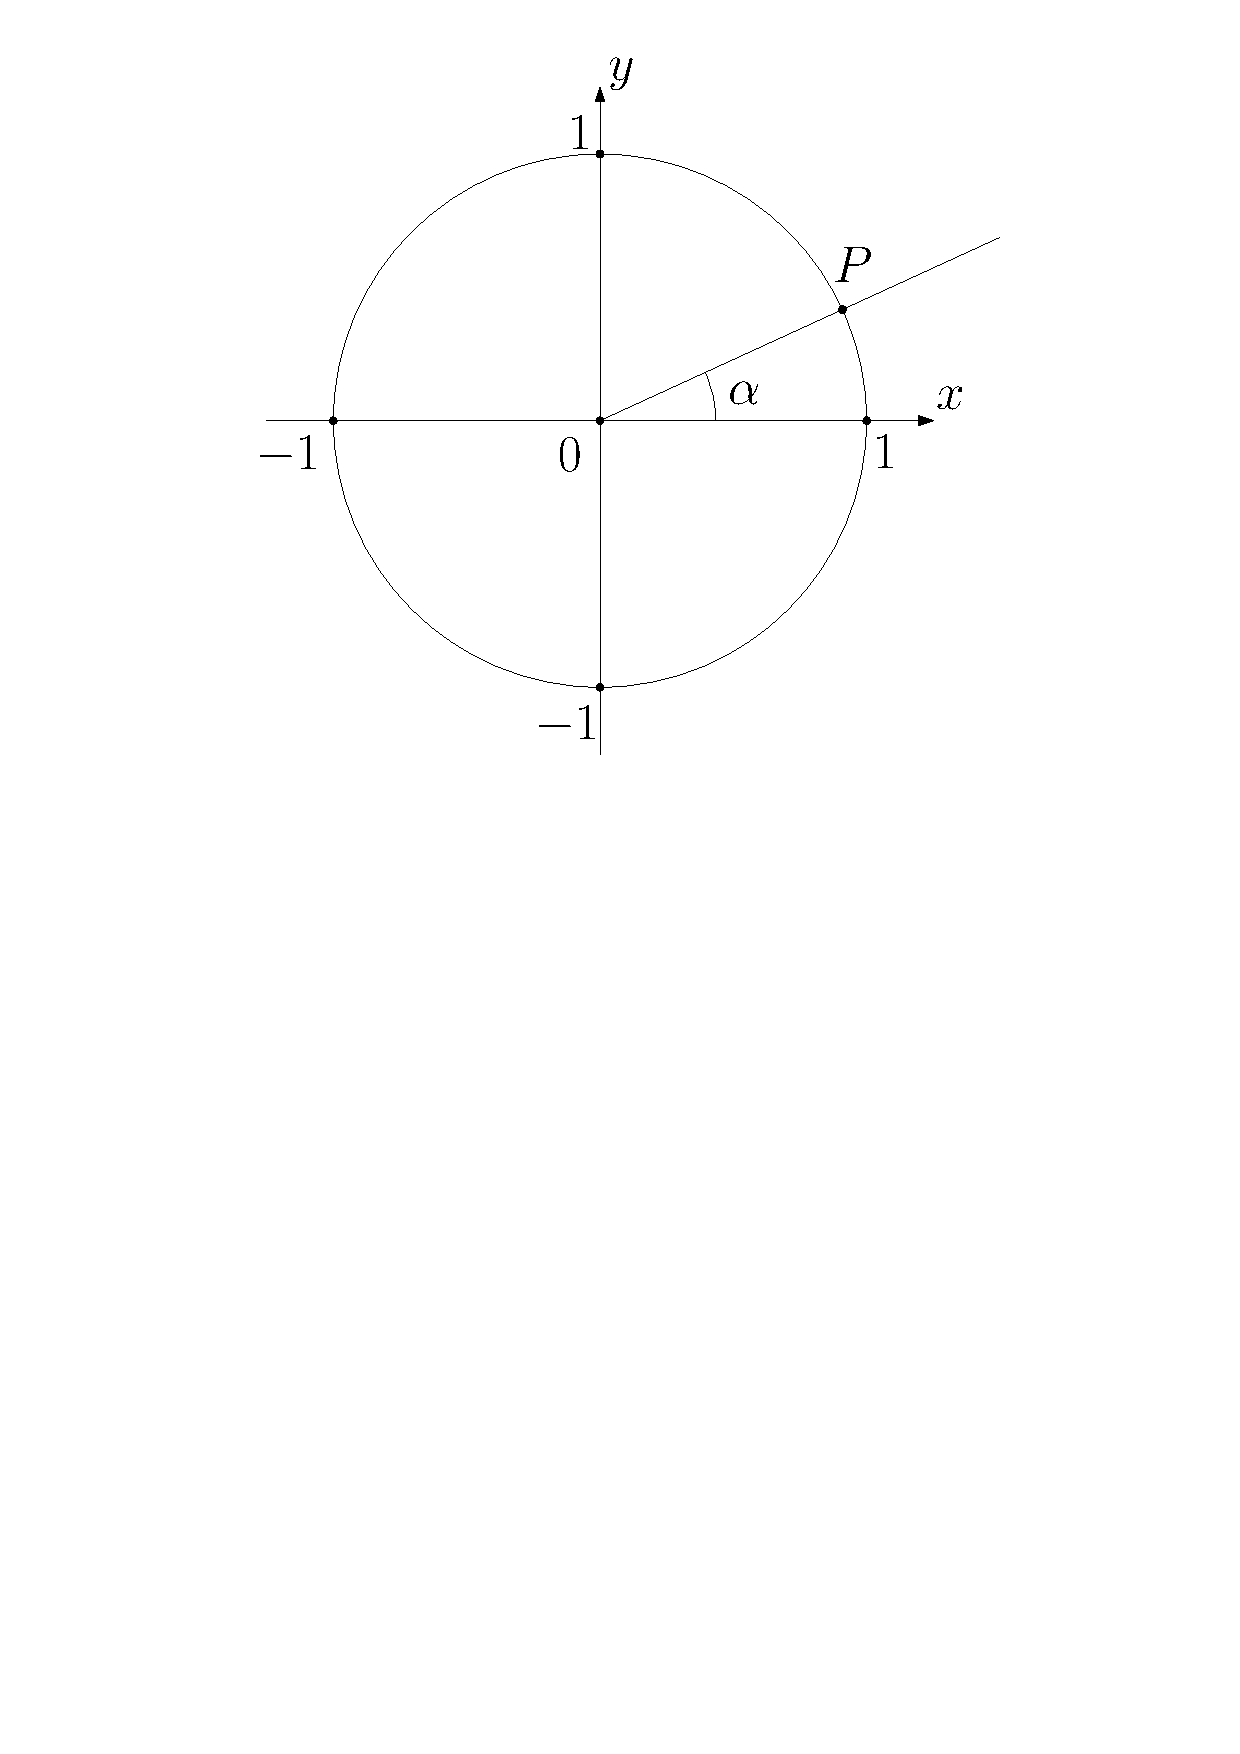
\includegraphics[scale=0.4]{3_gonio_complexe_getallen/inputs/goncirkelhoek.pdf}
\end{center}
\end{figure}

Je ziet dus dat elk punt dat je zou tekenen op de goniometrische cirkel, eigenlijk de voorstelling is van een hoek, door als beginbeen de $x$-as te nemen, als hoekpunt de oorsprong, en als eindbeen de halve rechte door de oorsprong en het punt.

\subsubsection{Goniometrische getallen}

We kennen de goniometrische getallen als verhoudingen van zijden in een rechthoekige driehoek:

\begin{align*}
\sin \alpha &= \frac{\textup{overstaande rechthoekszijde}}{\textup{schuine zijde}} &\qquad & \cos \alpha &= \frac{\textup{aanliggende rechthoekszijde}}{\textup{schuine zijde}}\\
&&\\
\tan \alpha &= \frac{\textup{overstaande rechthoekszijde}}{\textup{aanliggende rechthoekszijde}}&\qquad &\cot \alpha &= \frac{\textup{aanliggende rechthoekszijde}}{\textup{overstaande rechthoekszijde}}\\
\end{align*}

We kunnen een rechthoekige driehoek tekenen in de goniometrische cirkel, met zijden $a$, $b$ en $c$:

\gewonefiguur{scale=.5}{3_gonio_complexe_getallen/inputs/goncirkel3hoek.pdf}

%\begin{figure}[h]
%\begin{center}
%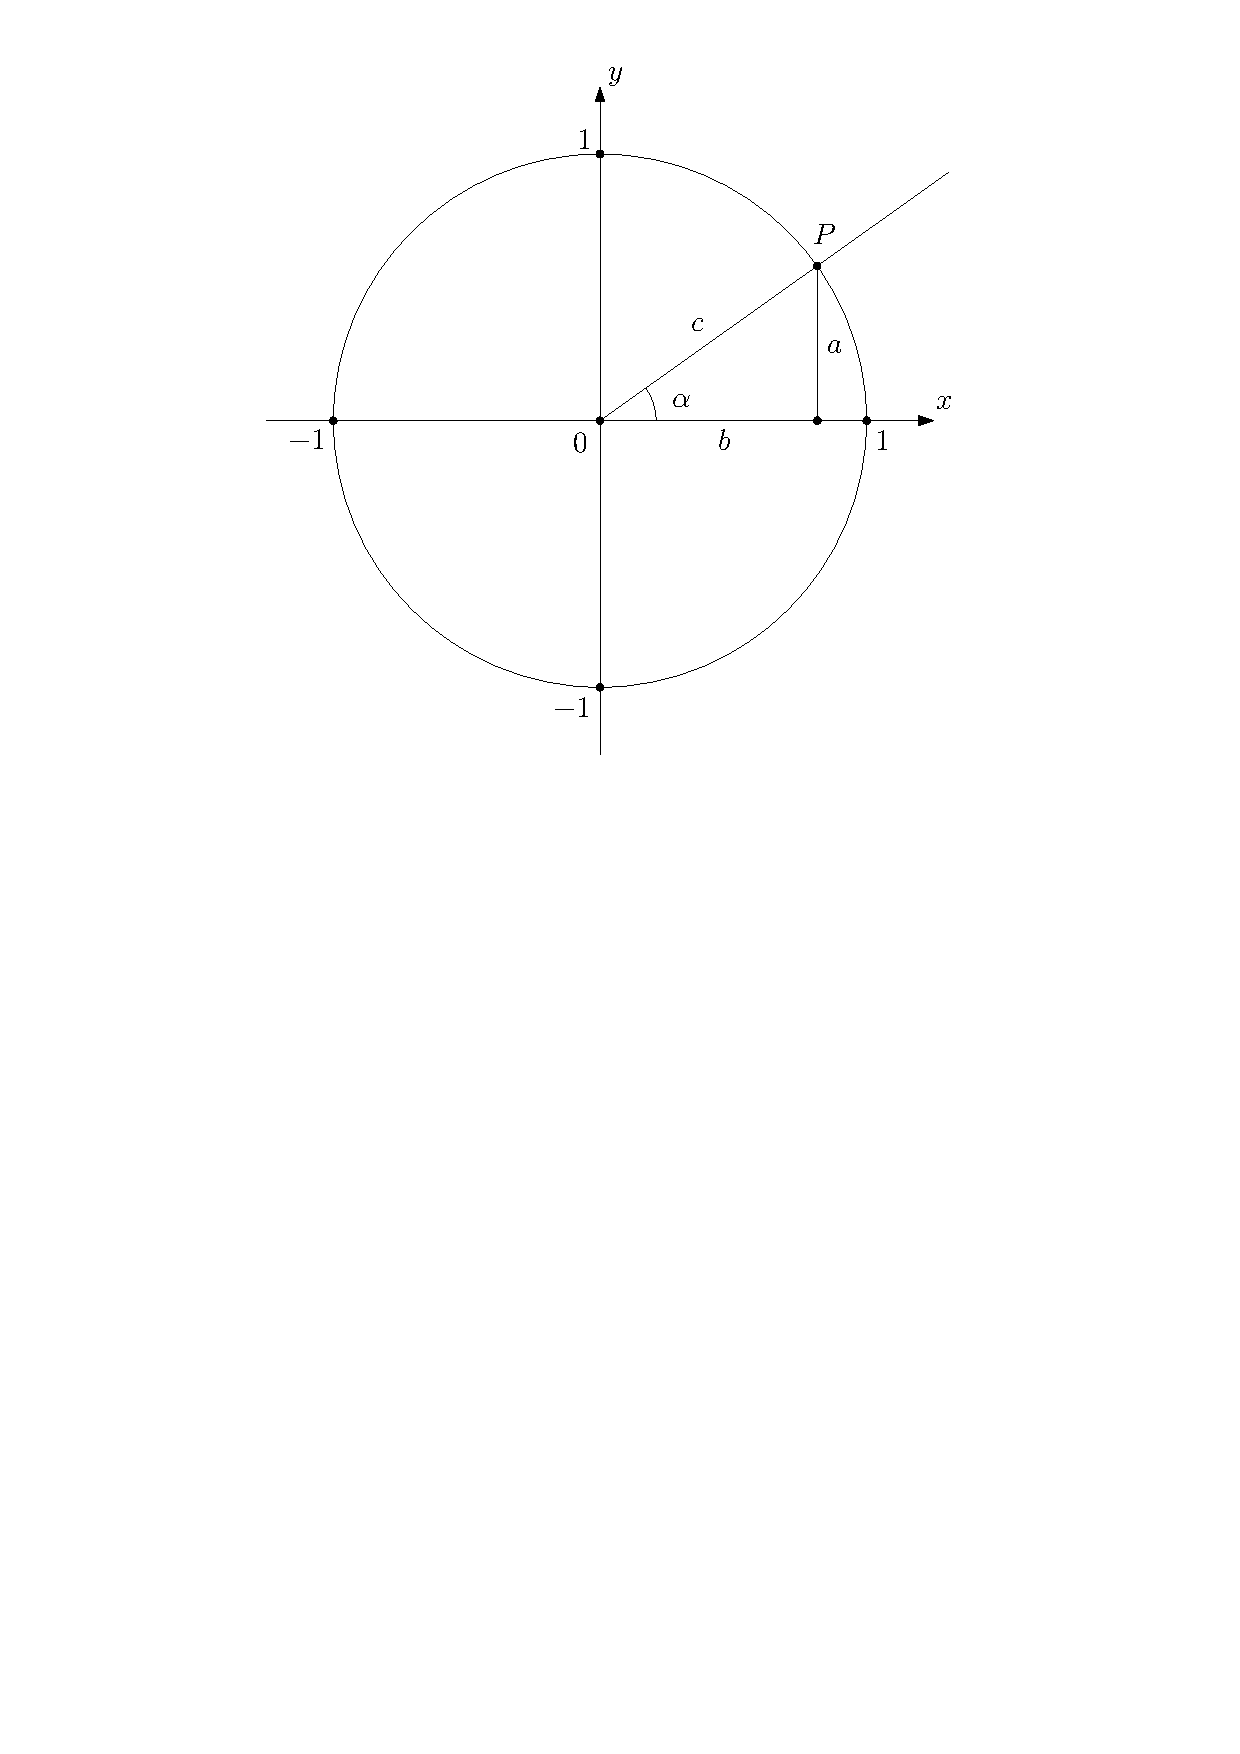
\includegraphics[scale=0.5]{3_gonio_complexe_getallen/inputs/goncirkel3hoek.pdf}
%\end{center}
%\end{figure}

In deze rechthoekige driehoek kan je nu de sinus en de cosinus berekenen:
\[\sin \alpha = \frac{a}{c} \qquad \cos \alpha = \frac{b}{c}\]
Je weet dat de lengte van zijde $c$ gelijk is aan $1$, omdat $c$ net de straal is van de goniometrische cirkel! Dus:
\[\sin \alpha = a \qquad \cos \alpha = b\]
De waarde van de sinus kan je dus aflezen op de $y$-as, en de waarde van de cosinus lees je af op de $x$-as, als je het punt $P$ ernaar projecteert.

\gewonefiguur{scale=.6}{3_gonio_complexe_getallen/inputs/goncirkelproj.pdf}

%\begin{center}
%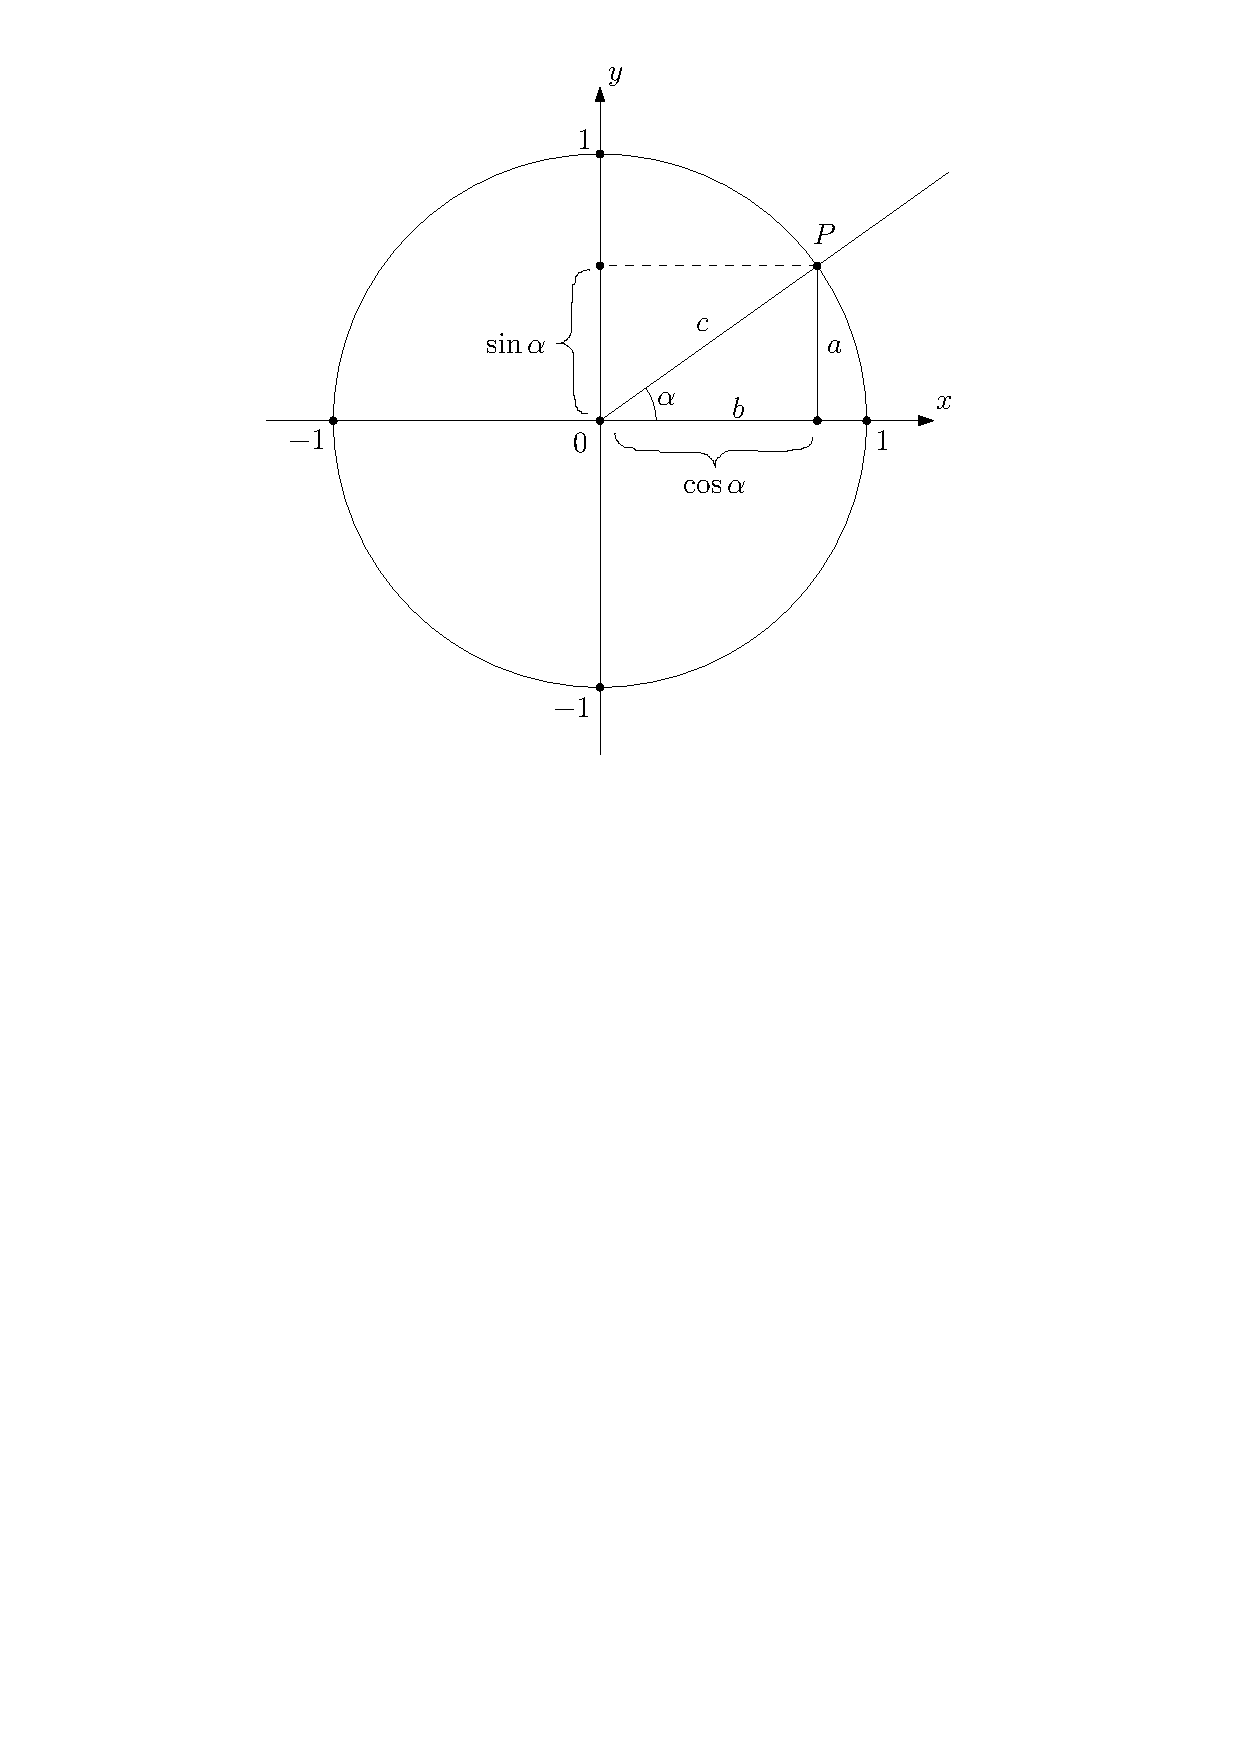
\includegraphics[scale=0.6]{3_gonio_complexe_getallen/inputs/goncirkelproj.pdf}
%\end{center}

Ook de tangens en cotangens kan je aflezen van de goniometrische cirkel.

\gewonefiguur{scale=.6}{3_gonio_complexe_getallen/inputs/goncirkeltancot.pdf}

%\begin{center}
%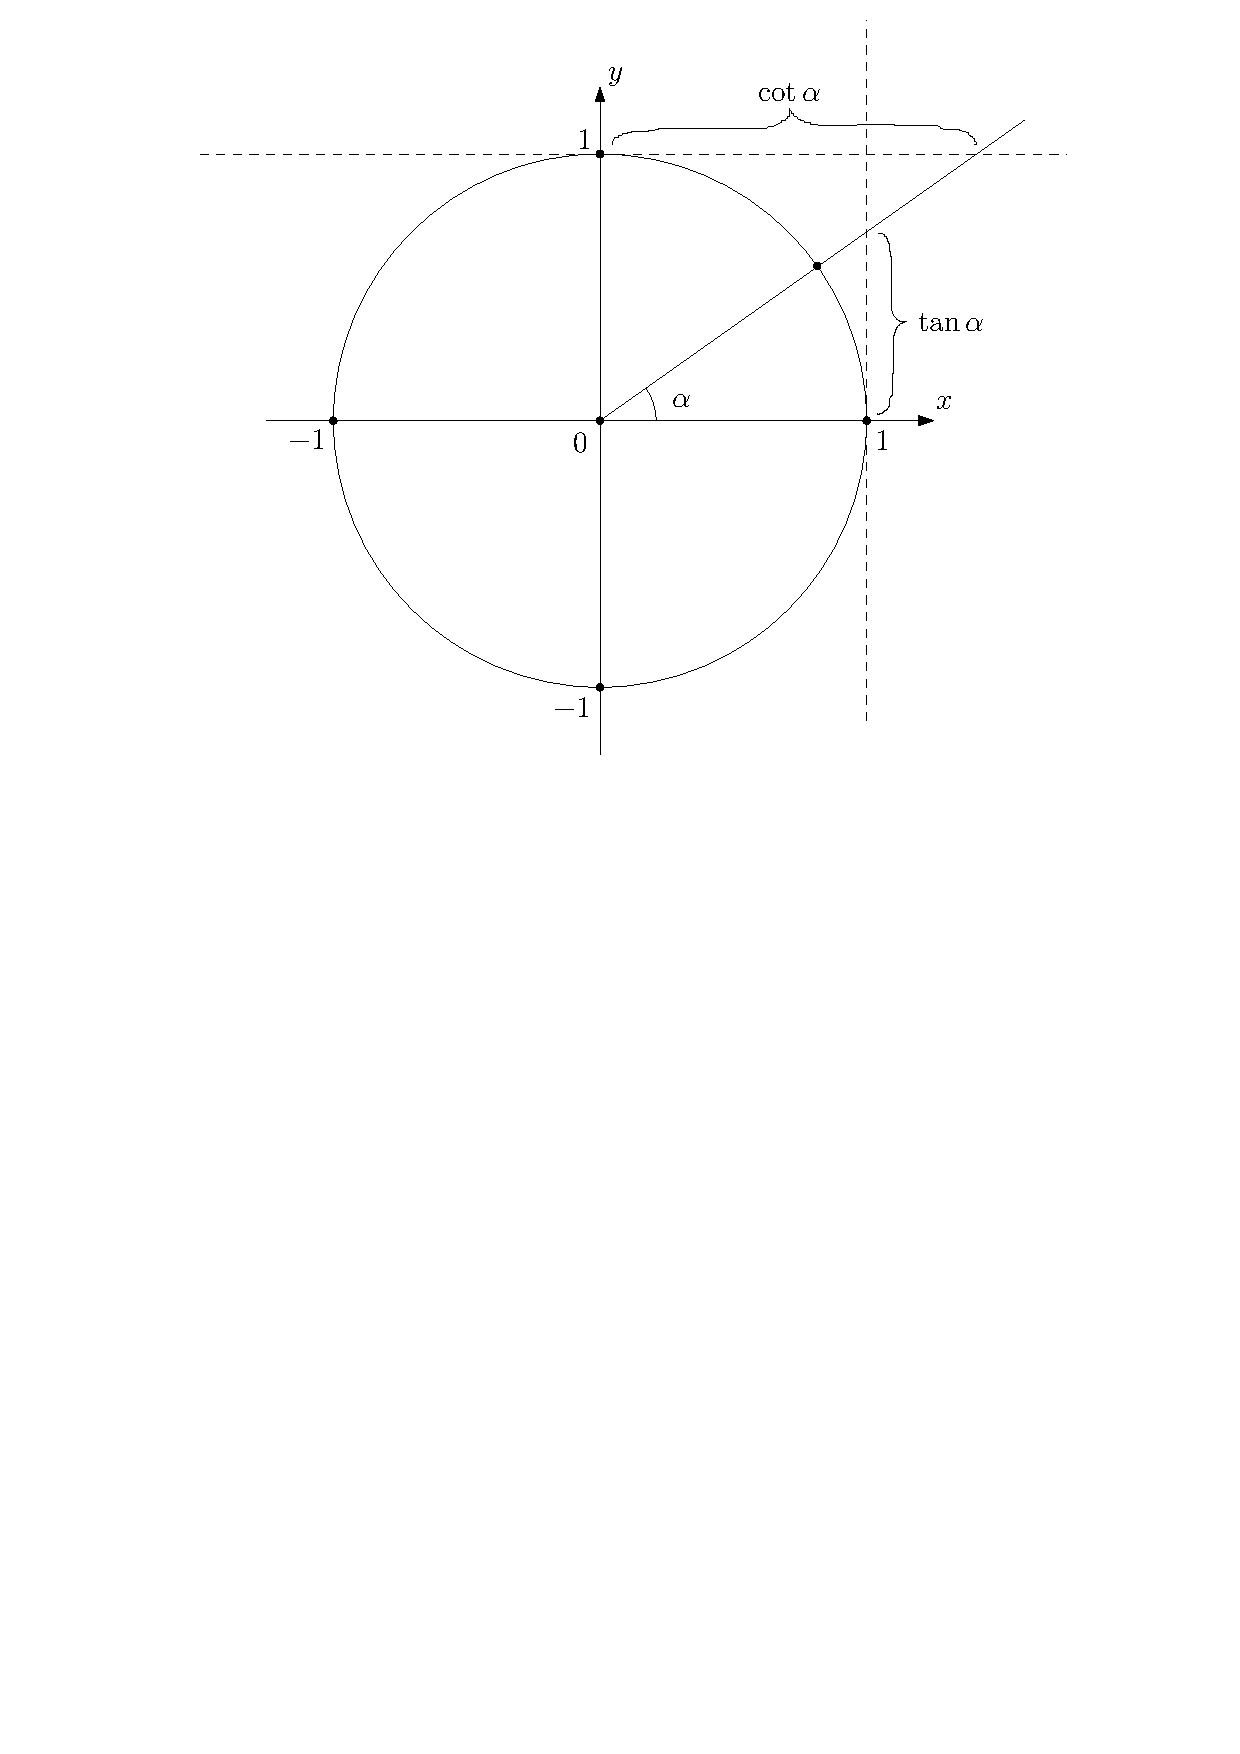
\includegraphics[scale=0.6]{3_gonio_complexe_getallen/inputs/goncirkeltancot.pdf}
%\end{center}

Uit deze twee figuren blijkt duidelijk dat de sinus en de cosinus niet kleiner kunnen zijn dan $-1$, en niet groter dan $1$. De tangens en de cotangens hebben deze beperkingen niet.

\subsubsection{Kwadranten}

De goniometrische cirkel wordt ingedeeld in kwadranten.

\gewonefiguur{scale=.5}{3_gonio_complexe_getallen/inputs/goncirkelkwadrant.pdf}

%\begin{figure}[h]
%\begin{center}
%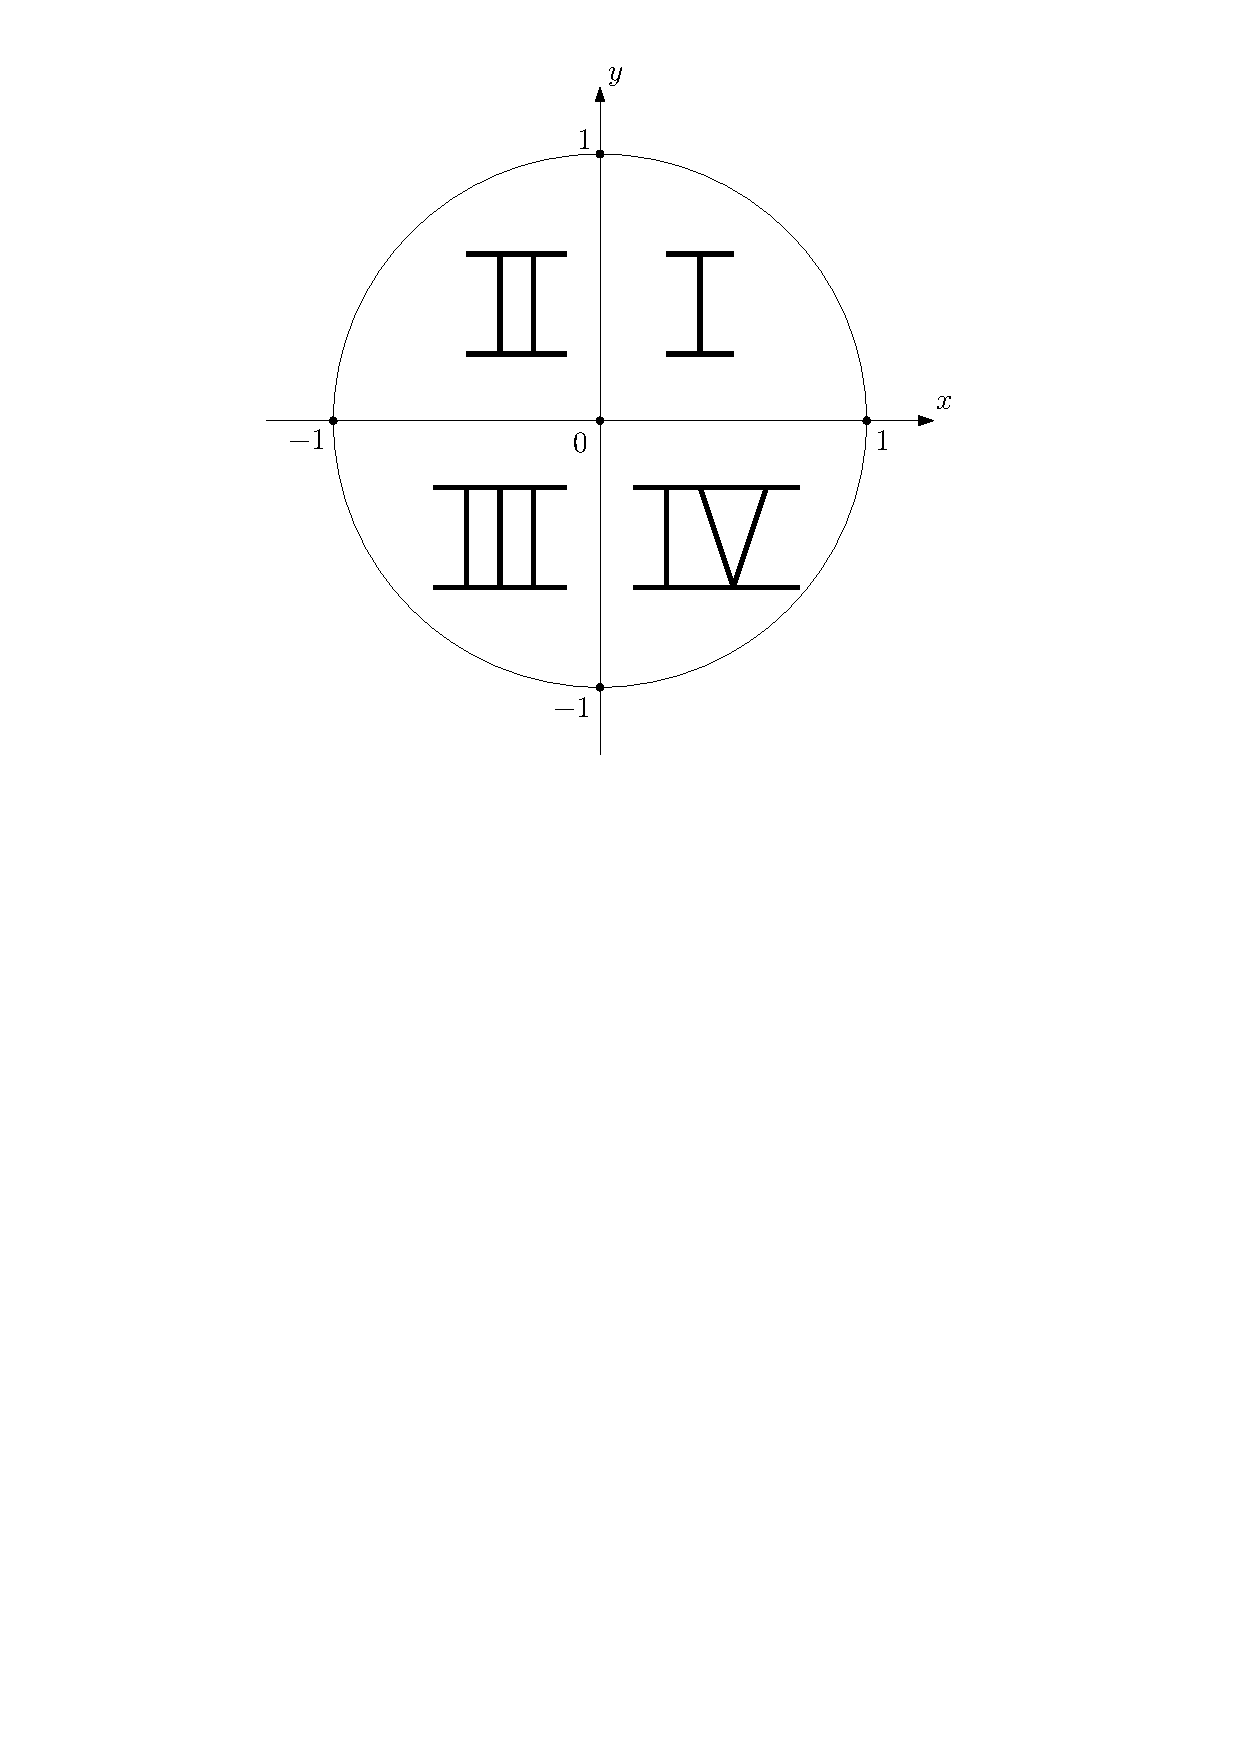
\includegraphics[scale=0.5]{3_gonio_complexe_getallen/inputs/goncirkelkwadrant.pdf}
%\end{center}
%\end{figure}

Ze zijn genummerd, meestal in Romeinse cijfers, tegenkloksgewijs, beginnend rechtsboven in de cirkel.
\begin{align*}
\alpha \in \textup{I} &\Leftrightarrow 0^\circ < \alpha < 90^\circ\\
\alpha \in \textup{II} &\Leftrightarrow 90^\circ < \alpha < 180^\circ\\
\alpha \in \textup{III} &\Leftrightarrow 180^\circ < \alpha < 270^\circ\\
\alpha \in \textup{IV} &\Leftrightarrow 270^\circ < \alpha < 360^\circ
\end{align*}
\begin{opmerking}
	 Bij het bespreken van willekeurige driehoeken hebben we vermeld dat het gebruik van het commando $\sin^{-1}$ op een rekentoestel om een hoek $\alpha$ te bepalen soms een verkeerd resultaat kan opleveren. Hieronder is op een figuur gedemonstreerd dat een hoek $\alpha$ uit het eerste kwadrant en een hoek $180^\circ -\alpha$ uit het tweede kwadrant dezelfde sinus hebben. De punten P en Q hebben immers dezelfde projectie op de Y-as.

\end{opmerking}

\gewonefiguur{scale=.5}{3_gonio_complexe_getallen/inputs/goncirkelproj-suppl.jpg}
%\begin{figure}[h]
%\begin{center}
%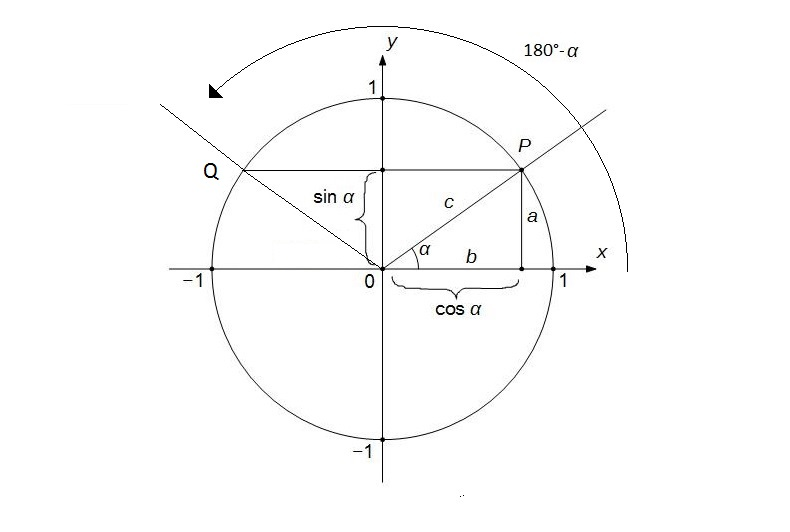
\includegraphics[scale=0.5]{3_gonio_complexe_getallen/inputs/goncirkelproj-suppl.jpg}
%\end{center}
%\end{figure}

\begin{onthoud}
	\ \\
	\begin{itemize}
	\item De goniometrische cirkel is een cirkel met straal $1$ door de oorsprong.
	\item Een hoek wordt weergegeven door een punt op de goniometrische cirkel. Het beginbeen is de positieve $x$-as, en het eindbeen door de rechte doro de oorsprong en dat punt op de goniometrische cirkel.
	\item De goniometrische getallen kan je aflezen van de goniometrische cirkel:
	\gewonefiguur{scale=.6}{3_gonio_complexe_getallen/inputs/goncirkeltotaal.pdf}
%	\begin{center}
%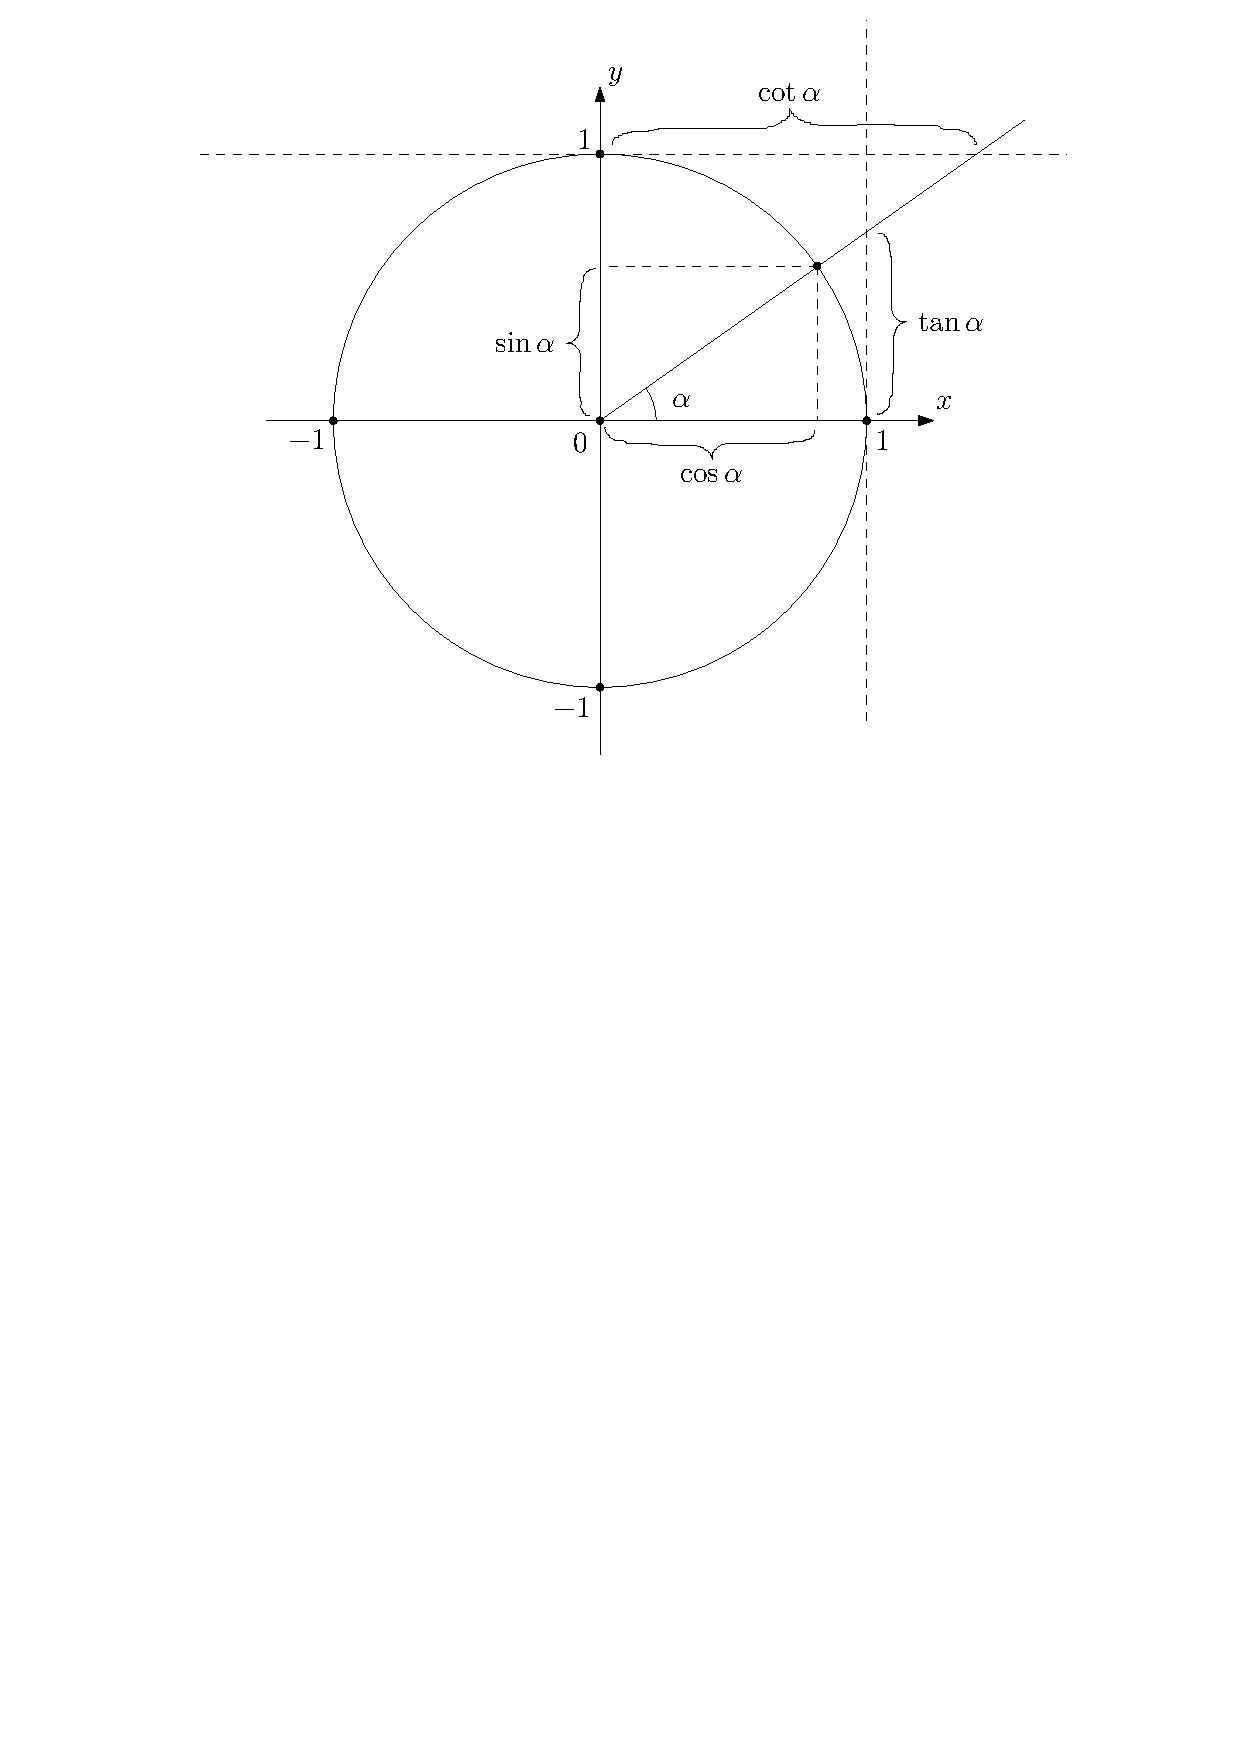
\includegraphics[scale=0.6]{3_gonio_complexe_getallen/inputs/goncirkeltotaal.pdf}
%\end{center}
	\item De kwadranten verdelen de goniometrische cirkels in $4$ sectoren:
	\gewonefiguur{scale=0.6}{3_gonio_complexe_getallen/inputs/goncirkelkwadrant.pdf}
%	\begin{center}
%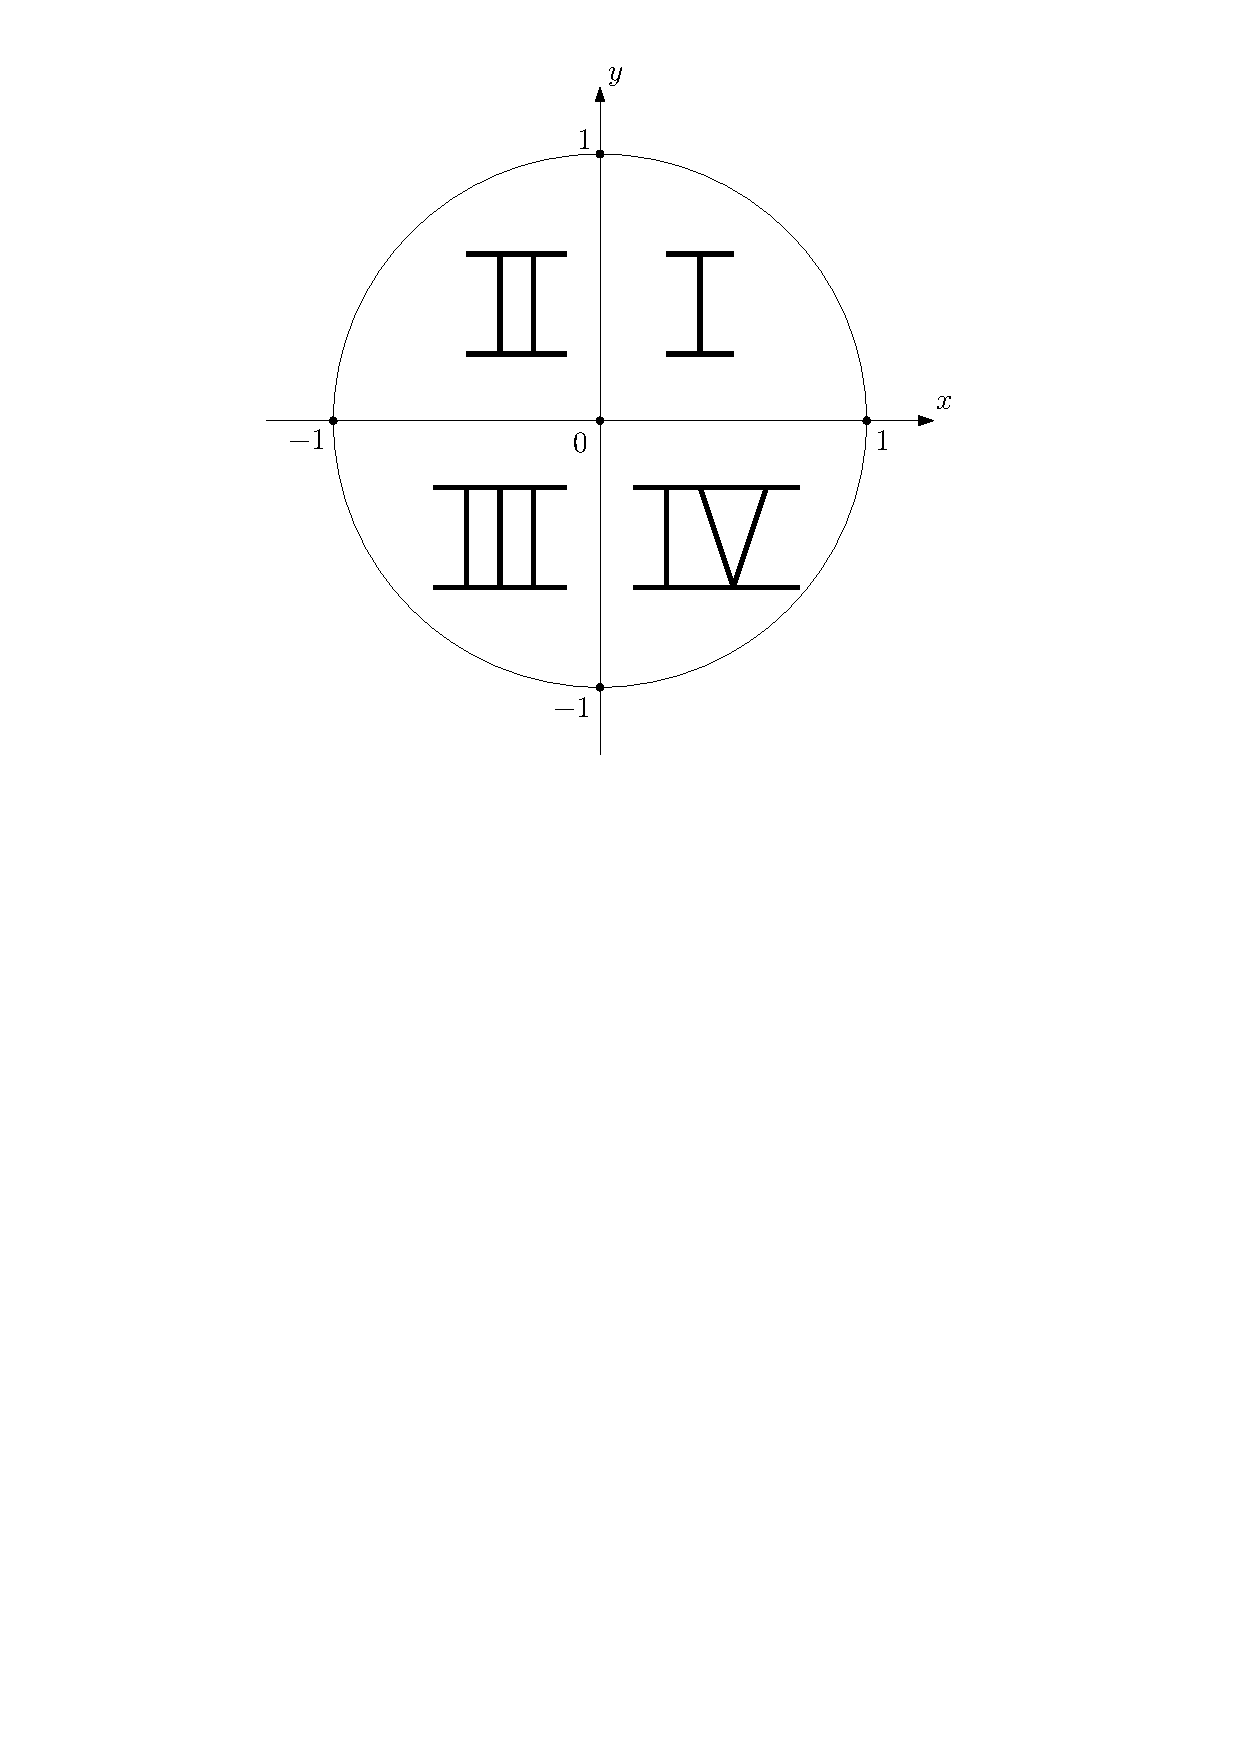
\includegraphics[scale=0.6]{3_gonio_complexe_getallen/inputs/goncirkelkwadrant.pdf}
%\end{center}
\begin{align*}
\alpha \in \textup{I} &\Leftrightarrow 0^\circ < \alpha < 90^\circ\\
\alpha \in \textup{II} &\Leftrightarrow 90^\circ < \alpha < 180^\circ\\
\alpha \in \textup{III} &\Leftrightarrow 180^\circ < \alpha < 270^\circ\\
\alpha \in \textup{IV} &\Leftrightarrow 270^\circ < \alpha < 360^\circ
\end{align*}
\end{itemize}

\end{onthoud}

\subsection{Goniometrische formules}

Dit hoofdstuk bestaat uit een opsomming van de belangrijkste formules in goniometrie.

\subsubsection{Bijzondere goniometrische getallen}

\begin{minipage}[b]{0.5\linewidth}
\begin{eqnarray*}
&&\tan \alpha = \frac{\sin \alpha}{\cos \alpha}\\
&&\\
&&\cot \alpha = \frac{\cos \alpha}{\sin \alpha}
\end{eqnarray*}
\end{minipage}
\hspace{0.5cm}
\begin{minipage}[b]{0.5\linewidth}
\begin{eqnarray*}
&&\textup{sec }\alpha = \frac{1}{\cos \alpha}\\
&&\\
&&\textup{csc }\alpha = \frac{1}{\sin \alpha}
\end{eqnarray*}
\end{minipage}

\subsubsection{Grondformules}

\begin{minipage}[b]{0.5\linewidth}
\begin{eqnarray*}
&&\cos^2\alpha +\sin^2 \alpha =1\\
&&1+\tan^2\alpha= \frac{1}{\cos^2 \alpha} = \sec^2 \alpha\\
&&1+\cot^2\alpha = \csc^2 \alpha
\end{eqnarray*}
\end{minipage}

\subsubsection{Verwante hoeken}
\vspace{0.2cm}
\begin{minipage}[b]{0.5\linewidth}
\textbf{Gelijke hoeken}
\begin{eqnarray*}
\sin(\alpha + k\cdot 360^\circ) &=& \sin(\alpha)\\
\cos(\alpha + k\cdot 360^\circ) &=& \cos(\alpha)\\
\tan(\alpha + k\cdot 360^\circ) &=& \tan(\alpha)\\
\cot(\alpha + k\cdot 360^\circ) &=& \cot(\alpha)
\end{eqnarray*}
\end{minipage}
\hspace{0.5cm}
\begin{minipage}[b]{0.5\linewidth}
\textbf{Tegengestelde hoeken}
\begin{eqnarray*}
\sin(-\alpha) &=& -\sin(\alpha)\\
\cos(-\alpha) &=& \cos(\alpha)\\
\tan(-\alpha) &=& -\tan(\alpha)\\
\cot(-\alpha) &=& -\cot(\alpha)
\end{eqnarray*}
\end{minipage}
\ \\
\begin{minipage}[b]{0.5\linewidth}
\textbf{Supplementaire hoeken}
\begin{eqnarray*}
\sin(180^\circ-\alpha) &=& \sin(\alpha)\\
\cos(180^\circ-\alpha) &=& -\cos(\alpha)\\
\tan(180^\circ-\alpha) &=& -\tan(\alpha)\\
\cot(180^\circ-\alpha) &=& -\cot(\alpha)
\end{eqnarray*}
\end{minipage}
\hspace{0.5cm}
\begin{minipage}[b]{0.5\linewidth}
\textbf{Antisupplementaire hoeken}
\begin{eqnarray*}
\sin(\alpha+180^\circ) &=& -\sin(\alpha)\\
\cos(\alpha+180^\circ) &=& -\cos(\alpha)\\
\tan(\alpha+180^\circ) &=& \tan(\alpha)\\
\cot(\alpha+180^\circ) &=& \cot(\alpha)
\end{eqnarray*}
\end{minipage}
\ \\
\begin{minipage}[b]{0.5\linewidth}
\textbf{Complementaire hoeken}
\begin{eqnarray*}
\sin\left(90^\circ-\alpha\right) &=& \cos(\alpha)\\
\cos\left(90^\circ-\alpha\right) &=& \sin(\alpha)\\
\tan\left(90^\circ-\alpha\right) &=& \cot(\alpha)\\
\cot\left(90^\circ-\alpha\right) &=& \tan(\alpha)
\end{eqnarray*}
\end{minipage}
\hspace{0.5cm}
\begin{minipage}[b]{0.5\linewidth}
\textbf{Anticomplementaire hoeken}
\begin{eqnarray*}
\sin\left(90^\circ+\alpha\right) &=& \cos(\alpha)\\
\cos\left(90^\circ+\alpha\right) &=& -\sin(\alpha)\\
\tan\left(90^\circ+\alpha\right) &=& -\cot(\alpha)\\
\cot\left(90^\circ+\alpha\right) &=& -\tan(\alpha)
\end{eqnarray*}
\end{minipage}

\subsubsection{Som- en verschilformules}

\begin{minipage}[b]{0.6\linewidth}
\begin{eqnarray*}
&&\sin(\alpha \pm \beta) = \sin\alpha\cos\beta \pm \cos\alpha\sin\beta\\
&&\cos(\alpha \pm \beta) = \cos\alpha\cos\beta \mp \sin\alpha\sin\beta\\
&&\tan(\alpha \pm \beta) = \frac{\tan\alpha\pm\tan\beta}{1\mp \tan\alpha\tan\beta} \\
&&\cot(\alpha \pm \beta) = \frac{\cot \alpha \cot\beta \mp 1}{\cot \alpha \pm \cot \beta}
\end{eqnarray*}
\end{minipage}

\subsubsection{Verdubbelingsformules}

\begin{minipage}[b]{0.5\linewidth}
\begin{eqnarray*}
\sin2\alpha &=& \frac{2\tan\alpha}{1+\tan^2\alpha}\\
\tan2\alpha &=& \frac{2\tan \alpha}{1-\tan^2\alpha}
\end{eqnarray*}
\end{minipage}
\hspace{0.5cm}
\begin{minipage}[b]{0.5\linewidth}
\begin{eqnarray*}
\cos2\alpha &=& \frac{1-\tan^2\alpha}{1+\tan^2\alpha}\\
&=& 1-2\sin^2\alpha\\
&=& 2\cos^2\alpha-1
\end{eqnarray*}
\end{minipage}

\subsubsection{Simpson-formules}

\begin{eqnarray*}
\sin(x)+\sin(y)&=&2\sin\frac{x+y}{2}\cos\frac{x-y}{2}\\
\sin(x)-\sin(y)&=&2\cos\frac{x+y}{2}\sin\frac{x-y}{2}\\
\cos(x)+\cos(y)&=&2\cos\frac{x+y}{2}\cos\frac{x-y}{2}\\
\cos(x)-\cos(y)&=&-2\sin\frac{x+y}{2}\sin\frac{x-y}{2}
\end{eqnarray*}

\subsubsection{Omgekeerde Simpson-formules}

\begin{eqnarray*}
\sin\alpha\cos\beta&=&\frac{1}{2}\left[\sin(\alpha + \beta)+\sin(\alpha - \beta)\right]\\
\cos\alpha\cos\beta&=&\frac{1}{2}\left[\cos(\alpha + \beta)+\cos(\alpha - \beta)\right]\\
\sin\alpha\sin\beta&=&-\frac{1}{2}\left[\cos(\alpha + \beta)-\cos(\alpha - \beta)\right]
\end{eqnarray*}

\subsection{Oefeningen}

\begin{oef}
	Druk uit in radialen:
	\begin{enumerate}
		\item $108,17^\circ$ 
		\item $12^\circ 40' 33''$ 
		\item $190$ gon
	\end{enumerate}
\end{oef}
\oplos{$1,887923$ rad; $0,221235$ rad; $2,984513$ rad (of ook: $\frac{19}{20}\pi$ rad)}

\begin{oef}
	Reken uit:
	\begin{enumerate}
		\item $267,83^\circ - 117,85^\circ$
		\item $12^\circ 02' 58'' + 4^\circ 13' 07''$
		\item $\frac{5}{3}\pi$ rad - $5^\circ 12' 57''$ (in radialen)
		\item $15,15$ gon + $15,15^\circ$ (in decimale graad)
	\end{enumerate}
\end{oef}
\oplos{$149,98^\circ$; $16^\circ 16' 05''$; $5,144954$ rad; $31,9833$ gon}

\subsubsection{Rekenen met driehoeken}

\begin{oef}
Om de hoogte van een mast te bepalen plaatst een landmeter een theodoliet in het punt $P$ op een hoogte $h=1,65$ m. Ze meet dan de hoeken $\alpha$ en $\beta$ met de horizontale: $\alpha=78,12^\circ$ en $\beta=4,71^\circ$.\\
Bereken de hoogte $H$ van de mast.

\gewonefiguur{scale=0.3}{3_gonio_complexe_getallen/inputs/oefn-mast.jpg}

%\begin{figure}[h]
%	\begin{center}
%		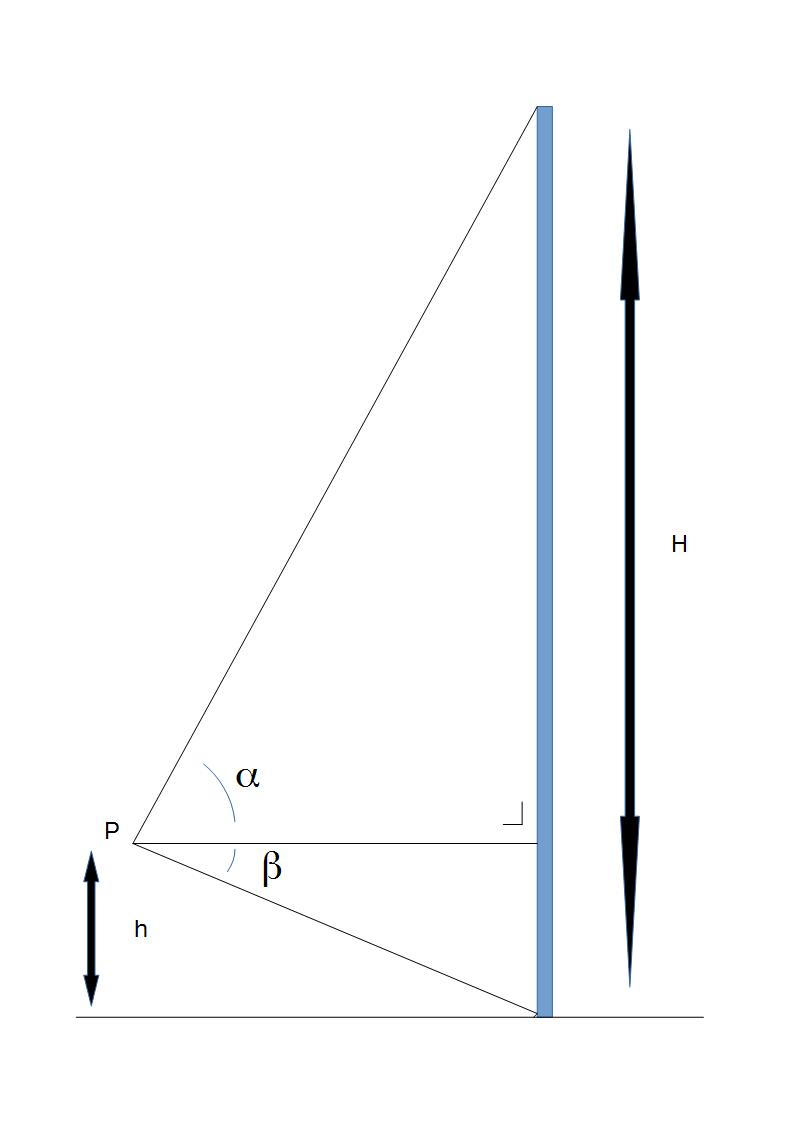
\includegraphics[scale=0.30]{\diepte/figures/oefn-mast.jpg}
%	\end{center}
%\end{figure}
\end{oef}
\oplos{$H=96,85$ m}

\begin{oef}
e lengte van elke zijde van de gegeven driehoek zijn gekend: $a=53$ cm, \\ $b=18$ cm en $c=41$ cm.\\
Bereken de hoek $\alpha$.

\gewonefiguur{scale=0.5}{3_gonio_complexe_getallen/inputs/oef-driehoek-1.jpg}
\end{oef}
\oplos{$\alpha=123,01^\circ$ }

\begin{oef}
Bereken de lengte van zijde $c$ van de gegeven driehoek.\\
Gegevens: $a=13$ mm, $b=20$ mm, $\alpha=21^\circ$. 

\gewonefiguur{scale=0.5}{3_gonio_complexe_getallen/inputs/oef-driehoek-2.jpg}
\end{oef}
\oplos{$c=7,83$ mm}

\begin{oef}
	Op de figuur is een schets van een stuk weiland met de gekende gegevens weergegeven. \\
	Bereken de lengte van zijde $d$ en de hoeken $\alpha$ en $\beta$.
	
	\gewonefiguur{scale=0.5}{3_gonio_complexe_getallen/inputs/oef-driehoek-3.jpg}
\end{oef}
\oplos{$d=33,17$ m; $\alpha=147,02^\circ$; $\beta=56,98^\circ$}


